\chapter{Instantiating the WSN construction}\label{ch:bison}
\marginpar{\vspace{-10pt}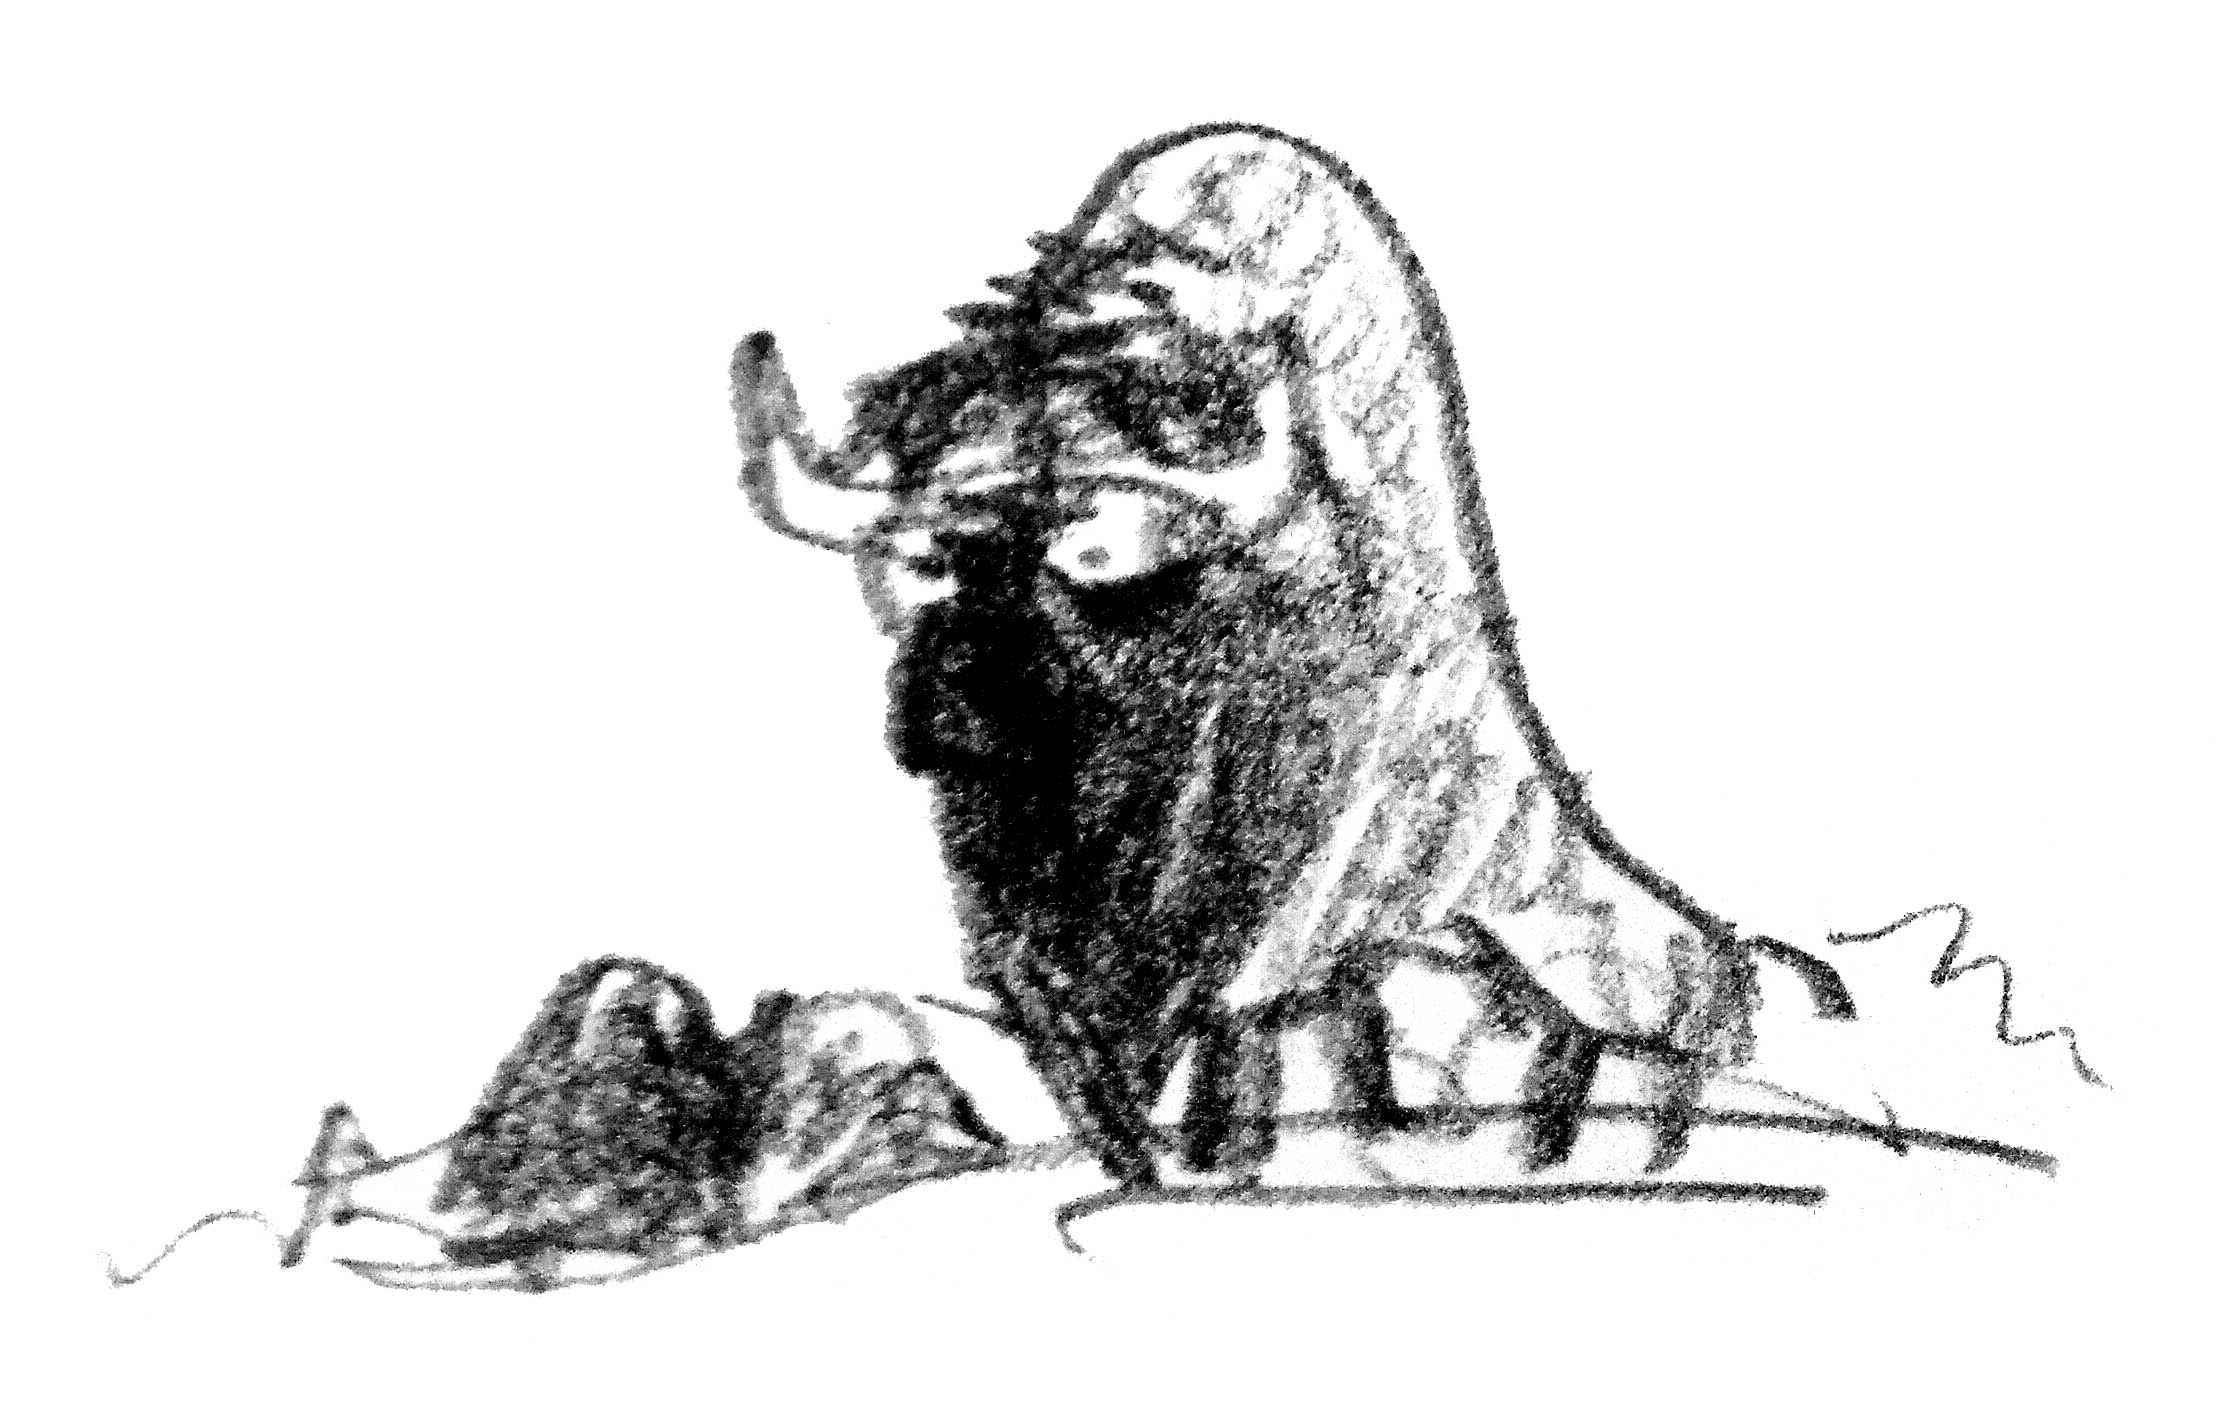
\includegraphics[width=52mm]{bison/bison-logo}\\\footnotesize\hphantom{.}\hfill---Lucas Hartmann}

\vspace*{-\baselineskip}
\newthought{Synopsis}\hspace{1.5em}
Our main contribution is a block cipher instance of the \WSN/ construction which allows us to give a strong bound on the best differential over several rounds of the cipher.
This chapter is based on the paper
\begin{quote}
    \fullfullcite{EC:CLLNW19}.
\end{quote}
All authors contributed equally.

After recalling the \WSN/ construction, we identify inherent restrictions and define a family of \WSN/ instances fulfilling these restrictions.
Subsequently, we discuss the differential cryptanalysis of these \enquote{\bison/-like} instances.
Following this analysis, we give two concrete species of \bison/-like block ciphers: \bison/ (with odd block length) and \wisent/ (with even block length).
For both we report on further cryptanalysis and give some remarks on implementation figures.

\section{Introduction}

In the context of \crefName{prob:cipher_constructions} an interesting result is the construction by \textcite{AC:Tessaro15}.
His construction is based on the Swap-or-Not construction by \textcite{C:HoaMorRog12}, which was designed for the setting where the component functions are secret.
Instead of being based on random permutations, this construction requires only a set of random (Boolean) functions.
Tessaro's construction, coined \WSNf/, requires only two public random (Boolean) functions $f_i$ with $n$-bit input, and can be proven to achieve full security, see \cref{sec:bison:wsn} for more details.

However, and this is the main motivation for our work, \emph{no instance of this construction is known}.
This situation is in sharp contrast to the case of the iterated Even-Mansour construction, where many secure instances are known for a long time already, as discussed in the previous chapter.

Without such a concrete instance, the framework of~\cite{AC:Tessaro15} remains of no avail.
As soon as one wants to use the framework in any way, one fundamentally has to instantiate the Boolean functions modeled as ideal functionalities by efficiently computable functions.
Clearly, the above mentioned bound in the ideal model does not say anything about any concrete instance.
Tessaro phrases this situation as follows:
\begin{quote}
    Heuristically, however, one hopes for even more: Namely, that under a careful implementation of the underlying component, the construction retains the promised security level.
    \hfill{}\cite{AC:Tessaro15}
\end{quote}

There has actually been one instance~\cite{C:HoaMorRog12} of the previous construction, but this has been broken almost instantaneously and completely, as parts of the encryption function were actually linear, see~\cite{C:Vaudenay12rump}.
This failure to securely instantiate the construction points to an important hurdle.
Namely, proving the generic bounds and analysing the security of an instance are technically very different tasks.
The security of any block cipher is with the current state of knowledge always the security against known attacks.
In particular, when designing any concrete block cipher, one has to argue why linear and differential attacks do not threaten the construction.

\newthoughtpar{Our Contribution}
Consequently, we investigate the important, but so far overlooked, aspect of instantiating the \WSN/ construction with a practical secure instance.
Practical secure meaning, just like in the case of \AES/, that the block cipher resists all known attacks.
We denote this instance as \bison/.\footnote{%
    For \enquote{Bent whItened Swap Or Not}
}
Our insights presented here are twofold.

First, we derive some inherent restrictions on the choice of the round function~$f_i$.
In a nutshell, we show that $f_i$ has to be rather strong, in the sense that its output bit has to basically depend on all input bits.
Moreover, we show that using less than $n$ rounds will always result in an insecure construction.
Those, from a cryptanalytic perspective rather obvious, results  are presented in \cref{bison:sec:restrictions}.
Again, but from a different angle, this situation is in sharp contrast to key-alternating ciphers.
In the case of key-alternating ciphers, even with a rather small number of rounds (\eg/~ten in the case of \AES/-128) and rather weak round functions (in case of the \AES/ round function any output bit depends on $32$~input bits only and the whole round function decomposes into four parallel functions on $32$~bits each) we get ciphers that provide, to the best of our knowledge today and after a significant amount of cryptanalysis, full security.

Second, despite those restrictions of the \WSN/ construction, that have significant impact on the performance of any instance, there are very positive aspects of the \WSN/ construction as well.
In \cref{bison:sec:dc}, we first define a family of \WSN/ instances which fulfill our initial restrictions.

As we will show in detail, this allows to argue very convincingly that our instance is secure against differential attacks.
Indeed, under standard assumptions, we can show that the probability of any (non-trivial) \emph{differential} is upper bounded by $2^{-n+1}$ where \(n\) is the block size, a value that is close to the ideal case.
% there exist no high probable {\emph{differential}} for any number of rounds $r\ge n$.
This significantly improves upon what is the state of the art for key-alternating ciphers.
As finding a solution to \crefName{prob:differentials} is notoriously hard, normally one therefore has to restrict to bounding the probability of \emph{differential characteristics} only.
Whereas our results for differential cryptanalysis gives a much simpler solution to \cref{prob:differentials}.
Additionally they can be of independent interest in the analysis of maximally unbalanced Feistel networks or nonlinear feedback shift registers.

We specify our concrete instance as a family of block ciphers for varying input length in \cref{sec:bison:instance}.
In our instance, we attach importance to simplicity and mathematical clarity.
It is making use of bent functions for instantiating $f$ and \LFSRp/ for generating the round keys.
Another advantage of \bison/ is that it defines a whole family of block ciphers, one for any odd block size.
In particular it allows the straightforward definition of small scale variants to be used for experiments.

Finally we discuss various other attacks and argue why they do not pose a threat for \bison/ in \cref{sec:bison:analysis}.
Particularly the discussion on algebraic attacks might be of independent interest.
For this we analyse the growth of the algebraic degree over the rounds.
In contrast to what we intuitively expect -- an exponential growth (until a certain threshold) as in the case for \SPNp/~\cite{FSE:BouCanDeC11} -- the degree of the \WSN/ construction grows linearly in the degree of the round function $f_i$.
This result can also be applied in the analysis of maximally unbalanced Feistel networks or nonlinear feedback shift registers.

Additionally to the results in~\cite{EC:CLLNW19}, we given an even block length instance, \wisent/, of the \WSN/ construction, see \cref{sec:wisent:instance}.
We conclude this section by adjusting our security and implementation analysis to this new instance.


\newthoughtpar{Related Work}
The first cipher, a Feistel structure, that allowed similarly strong arguments against differential attacks was presented by Nyberg and Knudsen~\cite{JC:NybKnu95}, see also~\cite{FSE:Nyberg12} for a nice survey on the topic.
This cipher was named CRADIC, as Cipher Resistant Against DIfferential Cryptanalysis but is often simply referenced as the KN cipher.
However, the cipher has been broken quickly afterwards, with the invention of interpolation attacks~\cite{FSE:JakKnu97}.
Another, technically very different approach to get strong results on resistance against attacks we would like to mention is the decorrelation theory~\cite{STACS:Vaudenay98}.
Interestingly, both previous approaches rely rather on one strong component, \ie/ round function, to ensure security, while the \WSN/ approach, and in particular \bison/, gains its resistance against differential attacks step by step.

Regarding the analysis of differentials, extensive efforts have been expended to evaluate the \MEDP//\MELP/ of \SPN/ ciphers, and in particular of the \AES/.
Some remarkable results were published by~\cite{FSE:PSLL03} and then subsequently improved by~\cite{IETIS:KelSui07} with a sophisticated pruning algorithm.
Interestingly, further work by~\cite{SCN:DaeRij06} and later by~\cite{EC:CanRou15} revealed that such bounds are not invariant under affine transformations.
All these works stress out how difficult it is to evaluate the \MEDP//\MELP/ of \SPNp/, even for a small number of rounds.
On the contrary, and as we are going to elaborate in the remaining of this paper, computing the \MEDP/ of \bison/ is rather straightforward and independent of the exact details of the components.
This can be compared to the wide trail strategy that, making use of the branch number and the superbox argument, allows bounding the probability of any differential characteristic for a large class of \SPNp/.
Our arguments allow to bound the differential probability for a large class of \WSN/ instances.

Before discussing our analysis in detail, we shortly recapitulate the \WSN/ construction.

\section{The Whitened Swap-or-Not construction}\label{sec:bison:wsn}

The \WSN/ construction is defined as follows.
Given two round keys $k_i$, $w_i$, the $i$-th round $R_{k_i,w_i}$ computes
\begin{align*}
    R_{k_i,w_i} : \F_2^n &\to \F_2^n \\
    R_{k_i,w_i}(x) &\coloneqq x + f_{b(i)}(w_i + \max\set{x, x + k_i}) \cdot k_i
\end{align*}
where $f_{0,1} : \F_2^n \to \F_2$ are modeled as two ideal random functions, the $\max$ function returns the lexicographic biggest value in the input set.
The index $b(i)$ equals zero for the first half of the rounds and one for the second half (see \cref{bison:fig:WSN} for a graphical overview of the encryption process).

In the remainder of the paper, we denote by $E_{k,w}^r(x)$ the application of $r$ rounds of the construction to the input $x$ with round keys $k_i$ and $w_i$ derived from the master key $(k,w)$.
Every round is involutory, thus for decryption one only has to reverse the order of the round keys.

\marginpar{%
    \centering
    \begin{tikzpicture}
        \node (input1) {$x$};

        \node (f1) [right=0.5em of input1, yshift=-1.5em] {$f_0$};
        \node (f1left) [left=0.5em of input1, yshift=-1.5em, color=white] {$f_0$};
        \draw [latex-latex] (f1left) edge[out=-45, in=-135, looseness=1.4] (f1);

        \draw (input1)
            -- +(0, -2.5em) node (f1split) {}
            -- +(1em, -3.5em) node [xshift=5pt] (f1_1) {\scriptsize $1$}
            -- +(1em, -5em) node [XOR, scale=0.8] (f1xor) {}
            -- (f1xor.center)
            -- +(0em, -1.5em)
            -- +(-1em, -2.5em) node (f1merge) {}
            -- +(-1em, -4em) node (input2) {};
        \draw [dashed] (f1split.center)
            -- +(-1em, -1em) node [xshift=-5pt] (f1_0) {\scriptsize $0$}
            -- +(-1em, -4em)
            -- (f1merge.center);

        \node (k1) [right=1.5em of f1xor] {$k_1$};
        \draw [-latex] (k1) -- ($(f1xor)+(8pt,0pt)$);


        \node (f2) [below=5.5em of f1] {$f_0$};
        \node (f2left) [below=5.5em of f1left, color=white] {$f_0$};
        \draw [latex-latex] (f2left) edge[out=-45, in=-135, looseness=1.4] (f2);

        \draw (input2.center)
            -- +(0, -0.5em) node (f2split) {};
        \draw [dashed] (f2split.center)
            -- +(1em, -1em) node [xshift=5pt] (f2_1) {\scriptsize $1$}
            -- +(1em, -2.5em) node [XOR, scale=0.8] (f2xor) {}
            -- (f2xor.center)
            -- +(0em, -1.5em)
            -- +(-1em, -2.5em) node (f2merge) {};
        \draw (f2merge.center)
            -- +(0em, -1em) node (output2) {};
        \draw (f2split.center)
            -- +(-1em, -1em) node [xshift=-5pt] (f2_0) {\scriptsize $0$}
            -- +(-1em, -4em)
            -- (f2merge.center);

        \node (k2) [right=1.5em of f2xor] {$k_2$};
        \draw [-latex] (k2) -- ($(f2xor)+(8pt,0pt)$);


        \node (dots) [below=-10pt of output2] {$\vdots$};

        \node (input3) [below=4pt of dots] {};

        \node (f3) [below=7em of f2] {$f_1$};
        \node (f3left) [below=7em of f2left, color=white] {$f_1$};
        \draw [latex-latex] (f3left) edge[out=-45, in=-135, looseness=1.4] (f3);

        \draw ($(input3.north)+(0,0.5em)$)
            -- +(0, -1em) node (f3split) {}
            -- +(1em, -2em) node [xshift=5pt] (f3_1) {\scriptsize $1$}
            -- +(1em, -3.5em) node [XOR, scale=0.8] (f3xor) {}
            -- (f3xor.center)
            -- +(0em, -1.5em)
            -- +(-1em, -2.5em) node (f3merge) {};
        \draw [-latex] (f3merge.center)
            -- +(0em, -1.5em) node (output4) {};
        \draw [dashed] (f3split.center)
            -- +(-1em, -1em) node [xshift=-5pt] (f3_0) {\scriptsize $0$}
            -- +(-1em, -4em)
            -- (f3merge.center);

        \node (k3) [right=1.5em of f3xor] {$k_r$};
        \draw [-latex] (k3) -- ($(f3xor)+(8pt,0pt)$);

        \node [below=-5pt of output4] {$E_{k,w}^r(x)$};
    \end{tikzpicture}
    \captionof{figure}{%
        Schematic view of the \WSNs/ construction.
    }\label{bison:fig:WSN}
}

Note that the usage of the maximum function is not decisive; it can be replaced by any function $\Phi_k$ that returns a unique representative of the set $\set{x, x+k}$, see~\citeonly{AC:Tessaro15}.
In other words it can be replaced by any function such that $\Phi_k(x) = \Phi_k(y)$ if and only if  $y \in \{x,x+k\}$.

The main result given by Tessaro on the security of the \WSN/ is the following (we only cite the informal statement, as our focus is not on the provable security aspect, but on practical instances).
\begin{proposition}[Security of the \WSN/ construction (Informal)~\citeonly{AC:Tessaro15}]
    The \WSN/ construction with $\Theta(n)$ rounds\footnote{%
        \citeauthor{AC:Tessaro15} claims security for $\mathcal{O}(n)$ rounds and notes that $\Omega(n)$ rounds are necessary to achieve information theoretically indistinguishability, as for a single query the internal Boolean function $f$ can only supply at most one bit of randomness.
    } is $(2^{n-\mathcal{O}(\log n)}, 2^{n-\mathcal{O}(1)} )$-secure.
\end{proposition}
Thus, any adversary trying to distinguish the \WSN/ construction from a random permutation and making at most $2^{n-\mathcal{O}(\log n)}$ queries to the block cipher and $2^{n-\mathcal{O}(1)}$ queries to the underlying function has negligible advantage.
Here, the round keys are modeled as independent and uniformly distributed random variables.

While \citeauthor{AC:Tessaro15}'s result gives us a strong security guarantee, the generic construction is not a practical instance.
Any practical block cipher has to provide security arguments against known attacks and, even more important, it has to give concrete details about the building blocks involved -- in this case the key schedule, the Boolean functions $f_0$ and $f_1$, and the actual number of rounds used.
To fill this gap between theory and practice here, we now analyse which generic properties any \WSN/ instance has to fulfill, and then give concrete instances of it.

\section{Inherent Restrictions}\label{bison:sec:restrictions}
In this section we point out two inherent restrictions on any practical secure instance.
Those restrictions result in general conditions on both the minimal number of rounds to be used and general properties of the round functions~$f_{b(i)}$.
In particular, those insights are taken into account for \bison/ and \wisent/.
While these restrictions are rather obvious from a cryptanalytic point of view, they have a severe impact on the performance of any concrete instance.
We discuss performance in more detail in \cref{sec:bison:implementation}.

\subsection{Number of Rounds}
As in every round of the cipher, we simply add (or not) the current round key~$k_i$, the ciphertext can always be expressed as the addition of the plaintext and a (message dependent) linear combination of all round keys $k_i$.
The simple but important observation to be made here is that, as long as the round keys do not span the full space, the block cipher is easily attackable.

Phrased in terms of linear cryptanalysis we start with the following lemma.
\begin{lemma}\label{lem:wsn:prob_one_mask}
    For any number of rounds $r<n$ there exists an element $u \in \F_2^n\setminus\{0\}$ such that
    \begin{equation*}
        \FC{E_{k,w}^r}(u,u)=2^n,
    \end{equation*}
    that is the equation
    \begin{equation*}
        \iprod{u}{x} = \iprod{u}{E_{k,w}^r(x)}
    \end{equation*}
    holds for all $x \in \F_2^n$.
\end{lemma}
\begin{proof}
    Let $k_1, \dots, k_{r}$ be the round keys derived from $k$ and denote by
    \begin{equation*}
        U = \Span{k_1, \dots, k_{r}}^{\perp}
    \end{equation*}
    the dual space of the space spanned by the round keys.
    As $r<n$ by assumption, the dimension of $\Span{k_1, \dots, k_{r}}$ is smaller than $n$ and thus $U \neq \set{0}$.
    Therefore, $U$ contains a non-zero element
    \begin{equation*}
        u \in \Span{k_1, \dots, k_{r}}^{\perp}
    \end{equation*}
    and it holds that
    \begin{equation*}
        \iprod{u}{E_{k,w}^r(x)}
        = \iprod{u}{(x + \sum_{i=1}^{r} \lambda_i k_i)}
        = \iprod{u}{x} + \iprod{u}{\sum_{i=1}^{r} \lambda_i k_i}
        = \iprod{u}{x}
    \end{equation*}
    concluding the proof.
\end{proof}

Even more importantly, this observation leads directly to a known plaintext attack with very low data-complexity.
Given a set of $t$ plaintext/ciphertext $(p_i,c_i)$ pairs, an attacker simply computes
\begin{equation*}
    V = \Span{p_i+c_i \given 1 \leqslant i \leqslant t} \subseteq \Span{k_j \given 1 \leqslant j \leqslant r}.
\end{equation*}
Given $t > r$  slightly more pairs than rounds, and assuming that $p_i+c_i$ is uniformly distributed in $\Span{k_j}$ (otherwise the attack only gets even stronger)\footnote{%
    For example if, with high probability, the $p_i + c_i$ do not depend on one or more $k_j$'s, the described attack can be extended to one or more rounds with high probability.
}
implies that
\begin{equation*}
    V= \Span{k_j}
\end{equation*}
with high probability and $V$ can be efficiently computed.
Furthermore, as above $\dim(\Span{k_j})$ is at most $r$, we have $V^{\perp} \ne \{0\}$.
Given any $u \ne 0$ in $V^\perp$ allows to compute one bit of information on the plaintext given only the ciphertext and particularly distinguish the cipher from a random permutation in a chosen-plaintext setting efficiently.

A similar argument shows the following:
\begin{lemma}\label{lem:wsn:zero_cor}
    For any number of rounds $r$ smaller than $2n-3$ there exist nonzero $\alpha$ and $\beta$, such that
    \begin{equation*}
        \widehat{E_{k,w}^r}(\alpha, \beta) = 0\;.
    \end{equation*}
\end{lemma}
\begin{proof}
    We restrict to the case $r \geqslant n$ as otherwise the statement follows directly from the lemma above.
    Indeed, from Parseval's equality, the fact that $\widehat{E_{k,w}^r}(\alpha, \alpha)=2^n$ implies that $\widehat{E_{k,w}^r}(\alpha, \beta)=0$ for all $\beta \neq \alpha$.
    Let $k_1, \ldots, k_{r}$ be the round keys derived from $k$ and choose non-zero elements $\alpha \ne \beta$ such that
    \begin{equation*}
        \alpha \in \Span{k_1, \dots, k_{n-2}}^{\perp} \qquad
        \text{and} \qquad
        \beta \in \Span{k_{n-1}, \dots, k_{r}}^{\perp}.
    \end{equation*}
    Note that, as $r \le 2n-3$ by assumption such elements always exist.
    Next, we split the encryption function in two parts, the first $n-2$ rounds $E_1$ and the remaining $r-(n-2)<n$ rounds $E_2$, i.e.
    \begin{equation*}
        E_{k,w}^r = E_2 \circ E_1.
    \end{equation*}
    We can compute the Fourier coefficient of $E_{k,w}^r$ as
    \begin{equation*}
        \FC{E_{k,w}^r}(\alpha,\beta)=\sum_{\gamma \in \F_2^n} \frac{\FC{E_1}(\alpha,\gamma)}{2^n} \cdot \frac{\FC{E_2}(\gamma,\beta)}{2^n}.
    \end{equation*}
    Now, the above lemma and the choices of $\alpha$ and $\beta$ imply that $\FC{E_1}(\alpha,\gamma) = 0$ for $\gamma \ne \alpha$ and  $\FC{E_2}(\gamma,\beta) = 0$ for $\gamma \ne \beta$.
    Recalling that $\alpha \ne \beta$ by construction concludes the proof.
\end{proof}

However, as the masks $\alpha$ and $\beta$ depend on the key, and unlike above there does not seem to be an efficient way to compute those, we do not see a direct way to use this observation for an attack.

Summarising the observations above, we get the following conclusion:
\begin{rationale}\label{rat:wsn:one}
    Any practical instance must iterate at least $n$ rounds.
    Furthermore, it is beneficial if any set of $n$ consecutive round keys are linearly independent.\footnote{%
        If (some) round keys are linearly dependent, \cref{lem:wsn:prob_one_mask,lem:wsn:zero_cor} can easily be extended to more rounds.
    }
\end{rationale}

After having derived basic bounds on the number of rounds for any secure instance, we move on to criteria on the round function itself.

\subsection{Round Function}
Here, we investigate a very basic criterion on the round function, namely dependency on all input bits, when the round function of $E^r_{k,w}$ is defined by
\begin{equation*}
    R_{k_i,w_i}(x) = x + f_{b(i)}(w_i + \max\set{x, x + k_i}) \cdot k_i\;.
\end{equation*}
Given the Boolean functions $f_{b(i)}:\F_2^n \to \F_2$, the question we would like to discuss is if it is necessary that the output bit of $f_{b(i)}$ has to depend on all input bits.
The function $f_{b(i)}$ depends on an input bit $j$ if there are two inputs $x,x'$ differing only in the $j$th bit such that $f_{b(i)}(x)\ne f_{b(i)}(x')$.
Otherwise the function is independent of the $j$th bit and we get
\begin{equation*}
    f_{b(i)}(x) = f_{b(i)}(x+e_j)
\end{equation*}
for all $x$.

We denote by $N(x) \coloneqq \set{i \given x[i] = 1}$ the index set of 1-bits in $x$, and by $\nu(x) \coloneqq \max N(x)$ the index of the highest 1-bit in $x$, in other words $\nu(x) = \floor{\log_2(x)}$, when interpreting $x \in \F_2^n$ as an integer.
For the main observation on this criterion, we first need the following lemma.
\begin{lemma}
\label{bison:lem:max_diff}
    Let $x, \delta \in \F_2^n$ and $k$ uniformly randomly drawn from $\F_2^n$.
    Then
    \begin{equation*}
        \Pr\bracket{\max\{x+\delta,x+\delta+k\}=\max\{x,x+k\}+\delta} \geqslant 1-2^{\nu(\delta)-n}.
    \end{equation*}
\end{lemma}
\begin{proof}
    The equality depends on the highest bit of $\delta$ where $x$ and $x + k$ differ, which is basically $\nu(k)$.
    We have
    \begin{equation*}
        \Pr\bracket{\max\{x+\delta,x+\delta+k\}=\max\{x,x+k\}+\delta} = \Pr\bracket{\delta[\nu(k)] = 0},
    \end{equation*}
    which can also be written as
    \begin{equation*}
        \Pr\bracket{\delta[\nu(k)] = 0}
        %= \Pr\bracket{\nu(k) \notin N(\delta)}
        = 1 - \Pr\bracket{\nu(k) \in N(\delta)}
        = 1 - \sum_{i \in N(\delta)} \Pr\bracket{\nu(k) = i}.
    \end{equation*}
    Further we have $\Pr\bracket{\nu(k) = i} = 2^{i-n-1}$ and thus
    \begin{equation*}
        1 - \sum_{i \in N(\delta)} \Pr\bracket{\nu(k) = i} = 1 - \sum_{i \in N(\delta)} 2^{i - n - 1} \geqslant 1 - 2^{\nu(\delta) - n},
    \end{equation*}
    which concludes the proof.
\end{proof}

As we will see next, the functions $f_{b(i)}$ have to depend virtually on all \emph{linear combinations of bits}.
In other words, it is required that the functions $f_{b(i)}$ have no (non-trivial) derivative equal to the all-zero function.

\begin{lemma}
    If there exists a $\delta\in\F_2^n$ such that
    \begin{equation*}
        f_{b(i)}(x) = f_{b(i)}(x+\delta)
    \end{equation*}
    for all $x$ and $i\in \set{0,1}$ then
    \begin{equation*}
        \Pr\bracket{E_{k,w}^r(x)+E_{k,w}^r(x+\delta)=\delta} \geqslant \parens{1-2^{\nu(\delta)-n}}^{r}
    \end{equation*}
    where the probability is over the input $x$ and the keys $k$ and $w$.
\end{lemma}
\begin{proof}
    From \cref{bison:lem:max_diff} we have that
    \begin{equation*}
        \Pr\bracket{\max\{x+\delta,x+\delta+k\}=\max\{x,x+k\}+\delta} \geqslant 1-2^{\nu(\delta)-n}.
    \end{equation*}
    Now, we get for one round
    \begin{equation*}
        R_{k_i,w_i}(x) = x + f_{b(i)}(w_i + \max\set{x, x + k_i}) \cdot k_i
    \end{equation*}
    by the assumption that $f_{b(i)}(x)=f_{b(i)}(x+\delta)$ for all $x$
    \begin{equation*}
        R_{k_i,w_i}(x+\delta)= R_{k_i,w_i}(x)+\delta
    \end{equation*}
    with the same probability.
    Thus, for $r$ rounds and uniformly chosen keys, we get
    \begin{equation*}
        \Pr\bracket{E_{k,w}^r(x)+E_{k,w}^r(x+\delta)=\delta} \geqslant \parens{1-2^{\nu(\delta)-n}}^{r}
    \end{equation*}
    by induction.
\end{proof}

As an example, considering the case $n=128$, $r$ rounds, and both $f_0$ and $f_1$ that do not depend on the most significant byte.
Thus, we can choose $\delta = e_{121}$ as a unit vector with $\nu(\delta)=121$ and get a differential probability of
\begin{equation*}
    \Pr\bracket{E_{k,w}^r(x)+E_{k,w}^r(x+\delta)=\delta} \geqslant \parens{1-2^{121-128}}^{r} \approx \parens{0.36}^{r/n}
\end{equation*}
which would completely compromise the scheme for a reasonable number of rounds.
In general this shows that as long as both $f_{b(i)}$ do not depend on almost all bits, the scheme is immediately broken by differential cryptanalysis.
Now, one might hope that one could craft functions $f_0$ and $f_1$ where, \eg/ $f_0$ depends only on the first $\frac{n}{2}$ bits and $f_1$ on the last $\frac{n}{2}$ bits to overcome this restriction.
However, while such a construction might be secure against basic differential cryptanalysis, it would still be completely broken by boomerang attacks~\cite{FSE:Wagner99}.
The main idea of boomerang attacks is to split the whole block cipher in two parts such that one has a high probable differential for the first part and a second high probable differential for the second part, which is exactly the situation one would end up here.

Thus, both functions independently have to virtually depend on all input bits, and we deduce the following.
\begin{rationale}\label{rat:wsn:two}
    For a practical instance, the functions $f_{b(i)}$ has to depend on all bits.
    Even more, for any $\delta \in \F_2^n$ the probability of
    \begin{equation*}
        f_{b(i)}(x)=f_{b(i)}(x+\delta)
    \end{equation*}
    should be close to $\frac{1}{2}$.
\end{rationale}

It is worth noticing that the analysis leading to this rationale applies to the original round function.
However, as pointed out in~\cite[Section~3.1]{AC:Tessaro15}, in the definition of the round function, we can replace the function
\begin{equation*}
    x \mapsto \max\set{x, x + k}
\end{equation*}
by any function $\Phi_k$ such that $\Phi_k(x)=\Phi_k(x+k)$ for all~$x$.
While the following sections will focus on the case when $\Phi_k$ is linear, we proved that \cref{rat:wsn:two} is also valid in this other setting.

Again, this should be compared to key-alternating ciphers, where usually not all output bits of a single round function depend on all input bits.
For example for \AES/ any output bit after one round depends only on $32$ input bits and for \present/ any output bit only depends on $4$ input bits.
However, while for key-alternating ciphers this does not seem to be problematic, and indeed allows rather weak round functions to result in a secure scheme, for the \WSN/ construction the situation is very different.

Before specifying our exact instance, we want to discuss differential cryptanalysis of a broader family of instances.

\section{Differential Cryptanalysis of \bison/-like instances}\label{bison:sec:dc}
We coin an instance of the \WSN/ construction \enquote{\bison/-like}, if it iterates at least $n$ rounds with linearly independent round keys $k_1, \ldots, k_n$ and applies Boolean functions $f_{b(i)}$ that depend on all bits, \ie/ fulfill \cref{rat:wsn:two}.
As explained in~\cite[Section~3.1]{AC:Tessaro15}, in order to enable decryption it is required that the Boolean functions $f_{b(i)}$ return the same result for both $x$ and $x+k$.
In the original proposition by Tessaro, this is achieved by using the $\max$ function in the definition of the round function.
Using this technique reduces the number of possible inputs for the $f_{b(i)}$ to $2^{n-1}$.
To simplify the analysis and to ease notation, we replace the $\max$ function with a \emph{linear function} $\Phi_k : \F_2^n \to \F_2^{n-1}$ with $\Ker \Phi_k = \set{0,k}$.
From now on, we assume that any \bison/-like instance uses such a $\Phi_k$ instead of the $\max$ function.
The corresponding round function has then the following form
\begin{equation}
  R_{k_i, w_i}(x) \coloneqq x + f_{b(i)} \parens{w_i + \Phi_{k_i}\parens{x}} k_i.\label{bison:eqn:wsn_instance0}
\end{equation}

With the above conditions, any \bison/-like instance of the \WSN/ construction inherits $f$'s resistance to differential cryptanalysis, as we show in the remainder of this section.
%In particular, basing the round function on bent functions together with the fact that any $n$ consecutive round keys are linearly independent by construction nicely adds to this analysis.

For our analysis, we make two standard assumptions in symmetric cryptanalysis as mentioned above: the \emph{independence of whitening round keys} $w_i$ and the \emph{hypothesis of stochastic equivalence} with respect to these round keys.
That is, we assume round keys $w_i$ to be independently uniformly drawn and the resulting \EDP/ to equal the differential probabilities averaged over all $w$.
In the following sections, we will argue why these assumptions do fit to our design and back up the results by practical experiments (see \textsc{Experimental Results} in \cref{subsec:bison-other-attacks} and
\cite[Appendix~B]{EPRINT:CLLNW18}
%\cref{bison:app:figures}
).
For the round keys $k_i$ we do not have to make such assumptions.

We first discuss the simple case of differential behaviour for one round only and then move up to an arbitrary number of rounds and devise the number of possible output differences and their probabilities.

%In all that follows, we are interested in the EDP over all the possible $w_i$ for fixed keys $k_i$.

\subsection{From One-Round Differential Characteristics}
%Let $R_{k,w}$ denote the round function of a \bison/-like instance.
%Then, as the round function is bijective, the possible output differences for any input difference $\alpha \neq 0$ are clearly restricted to either $\alpha$, or $\alpha + k$.
Looking only at one round, we can compute the \DDT/ explicitly:

\begin{proposition}\label{prop:wsn:ddt}
    Let $R_{k_i,w_i} : \F_2^n \to \F_2^n$ be the \WSN/ round function as in \cref{bison:eqn:wsn_instance0}.
    Then its \DDT/ consists of the entries
    \begin{equation}
        \mathrm{\DDTs/}[\alpha,\beta] = \begin{cases*}
            2^{n-1} + \AC{f}(\Phi_k(\alpha)) & if $\beta = \alpha$  \\
            2^{n-1} - \AC{f}(\Phi_k(\alpha)) & if $\beta = \alpha+k$\\
                    0                        & otherwise
            \end{cases*}\;.
    \end{equation}
    \marginpar{\vspace{-4.5\baselineskip}\footnotesize$\AC{f}(\cdot)$ denotes the autocorrelation of $f$.}
    Most notably, if $f$ is bent, we have
    \begin{equation*}
        \mathrm{\DDTs/}[\alpha,\beta] = \begin{cases*}
            2^n     & if $\alpha = \beta = k$ or $\alpha = \beta = 0$ \\
            2^{n-1} & if $\beta \in \set{\alpha, \alpha + k}$ and $\alpha \not \in \Span{k}$\\
            0       & otherwise
        \end{cases*}\;.
    \end{equation*}
\end{proposition}
\begin{proof}
    We have to count the number of solutions of $R(x) + R(x + \alpha) = \beta$:
    \begin{align*}
        \mathrm{\DDTs/}[\alpha,\beta] & = \abs{\set{x \in \F_2^n \given R(x) + R(x + \alpha) = \beta}}\\
                                      & = \abs{\set{x \in \F_2^n \given \alpha + \left[f( w + \Phi_k(x)) + f( w + \Phi_k(x + \alpha))\right] \cdot k = \beta}}
    \end{align*}
    Since $f$ takes its values in $\F_2$, the only output differences $\beta$ such that $\text{\DDTs/}[\alpha,\beta]$ may differ from~$0$ are $\beta=\alpha$ and $\beta=\alpha +k$.
    When $\beta=\alpha$, we have
    %Thus we need to show that the number of $x$ for which $\Delta_\alpha(f)(x) = 0$, this is the case of $\alpha = \beta$, is either $2^n$ if $\Phi_k(\alpha) = 0$, or $2^{n-1}$ else.
    %Then the second part, there are exactly $2^{n-1}$ many $x$ for which the derivative is one and thus $\beta = \alpha + k$, follows directly.
    %f(w + \Phi_k(x)) + f(w + \Phi_k(x + \alpha)) = 0$
    \begin{align*}
        \mathrm{\DDTs/}[\alpha,\alpha] & = \abs{\set{x \in \F_2^n \given f( w + \Phi_k(x)) + f( w + \Phi_k(x + \alpha)) = 0}} \\
                                       & = \abs{\set{x \in \F_2^n \given f( w + \Phi_k(x)) + f( w + \Phi_k(x) + \Phi_k(\alpha)) = 0}} \\
                                       & = 2 \cdot \abs{\set{x^\prime \in \F_2^{n-1} \given f(x^\prime) + f(x^\prime + \Phi_k(\alpha)) = 0}} \\
                                       & = 2 \parens{2^{n-2} + \frac{1}{2} \widehat{\Delta_{\Phi_k(\alpha)}(f)}(0)} = 2^{n-1} + \AC{f}(\Phi_k(\alpha))\;.
    \end{align*}
    Similarly,
    \begin{align*}
        \mathrm{\DDTs/}[\alpha,\alpha+k] & = \abs{\set{x \in \F_2^n \given f( w + \Phi_k(x)) + f( w + \Phi_k(x + \alpha)) = 1}} \\
                                         & = 2 \parens{2^{n-2} - \frac{1}{2} \widehat{\Delta_{\Phi_k(\alpha)}(f)}(0)} = 2^{n-1} - \AC{f}(\Phi_k(\alpha))\;.
    \end{align*}
    Most notably, when $\alpha \in \set{0,k}$, $\AC{f}(\Phi_k(\alpha)) = \AC{f}(0) = 2^{n-1}$.
    Moreover, when $f$ is bent, $\AC{f}(\Phi_k(\alpha)) = 0$ for all other values of $\alpha$.
\end{proof}

\subsection{To Differentials over more Rounds}
As previously explained, it is possible to estimate the probability of a differential characteristic over several rounds, averaged over the round keys, when the cipher is a Markov cipher.
We now show that this assumption holds for any \bison/-like instance of the \WSN/ construction.

\begin{lemma}
    Let $R_{k,w} : \F_2^n \to \F_2^n$ be the \WSN/ round function as in \cref{bison:eqn:wsn_instance0}.
    For any fixed $k \in \F_2^n$ and any differential $\propDiff{\alpha}{}{\beta}$, we have that
    \begin{equation*}
        \Prob_w \left[R_{k,w}(x+\alpha) + R_{k,w}(x) =\beta\right]
    \end{equation*}
    is independent of~$x$.
    More precisely
    \begin{equation*}
        \Prob_w \left[R_{k,w}(x+\alpha) + R_{k,w}(x) =\beta\right] = \Prob_x \left[R_{k,w}(x+\alpha) + R_{k,w}(x) =\beta\right]\;.
    \end{equation*}
\end{lemma}
\begin{proof}
    We have
    \begin{align*}
           &\set{w \in \F_2^{n-1} \given \Delta_\alpha (R_{k,w})(x)=\beta} \\
        =\ &\set{w \in \F_2^{n-1} \given \parens{\Delta_{\Phi_k(\alpha)}(f)(w+\Phi_k(x))} \cdot k = \alpha + \beta}\\
        =\ &\begin{cases*}
            \emptyset & if $\beta \not \in \set{\alpha, \alpha+k}$\\
            \Phi_k(x) + \supp{\Delta_{\Phi_k(\alpha)}(f)} & if $\beta=\alpha + k$\\
            \Phi_k(x) + \parens{\F_2^{n-1} \setminus \supp{\Delta_{\Phi_k(\alpha)}(f)}} & if $\beta=\alpha$
        \end{cases*}\;.
    \end{align*}
    Clearly, the cardinality of this set does not depend on $x$. Moreover, this cardinality, divided by $2^{n-1}$, corresponds to the value of
    \begin{equation*}
        \Prob_x \bracket{R_{k,w}(x+\alpha) + R_{k,w}(x) =\beta}
    \end{equation*}
    computed in the previous proposition.
\end{proof}
By induction on the number of rounds, we then directly deduce that any \bison/-like instance of the \WSN/ construction is a Markov cipher in the sense of the following corollary.
\begin{corollary}\label{bison:coro:Markov}
    Let $E_{k,w}^i$ denote $i$~rounds of a \bison/-like instance of the \WSN/ construction with round function $R_{k_i,w_i}$.
    For any number of rounds~$r$ and any round keys $(k_1, \ldots, k_r)$, the probability of an $r$-round characteristic $\theta$ satisfies
    \begin{gather*}
            \Prob_{w}\bracket{E^i_{k,w}(x) + E^i_{k,w}(x+\theta_0)=\theta_i, \forall 1 \leqslant i \leqslant r} \\
            = \quad \prod_{i=1}^r \Prob_{x} \bracket{R_{k_i,w_i}(x) + R_{k_i,w_i}(x+\theta_{i-1}) = \theta_i}\;.
    \end{gather*}
\end{corollary}
%\ac{Maybe this proof is not needed since it is clear from the lemma?}
%\begin{proof}
%  By induction on~$r$. The case $r=1$ corresponds to the previous lemma. Let us now assume that the formula holds for any $(r-1)$-round characteristic $\delta$. The probability of the characteristic $(\delta, \delta_r)$ over $r$~rounds, $P(\delta, \delta_r)$, is given by
%  \begin{eqnarray*}
%    P(\delta, \delta_r) & = & \Prob_w \left[R_{k_r,w_r}(x_r) + R_{k_r,w_r}(x_r+\delta_{r-1})=\delta_r | x_r = E_{k,w}^{r-1}(x) \right.\\
%      & & \left.\quad \mbox{ and } E_{k,w}^{i}(x) + E_{k,w}^i(x+\delta_0) = \delta_i \forall 1 \leq i < r \right] \times P(\delta)\\
%        & = & \Prob_{w_r} \left[R_{k_r,w_r}(x_r) + R_{k_r,w_r}(x_r+\delta_{r-1})=\delta_r \right] \times P(\delta)\\
%         & = & \Prob_x \left[R_{k_r,w_r}(x) + R_{k_r,w_r}(x+\delta_{r-1})=\delta_r \right] \times P(\delta)\\
%  \end{eqnarray*}
%  where we use the fact that the probability over~$w_r$ of a one-round differential does not depend on~$x_r$.
%  \end{proof}

For many ciphers several differential characteristics can cluster in a \emph{differential} over more rounds.
This is the main reason why bounding the probability of differentials is usually very difficult if possible at all.
For \bison/-like instances the situation is much nicer; we can actually compute the \EDP/, \ie/ the probabilities of the differentials averaged over all whitening key sequences $(w_1, \ldots, w_r)$.
This comes from the fact that any differential for less than $n$ rounds contains at most one differential characteristic with non-zero probability.
To understand this behaviour, let us start by analysing the \EDP/ (averaged over the $w_i$) and by determining the number of possible output differences.

In the following, we assume that the input difference $\alpha$ is fixed, and we calculate the number of possible output differences.
We show that this quantity depends on the relation between $\alpha$ and the $k_i$.

\begin{lemma}\label{bison:lem:number_diffs}
    Let us consider $r$~rounds of  a \bison/-like instance of the \WSN/ construction with round function involving Boolean functions $f_{b(i)}$ having no (non-trivial) constant derivative.
    Assume that the first $n$ round keys $k_1, \dots, k_n$ are linearly independent, and that $k_{n+1}=k_1 + \sum_{i=2}^n \gamma_i k_i$ for $\gamma_i \in \F_2$.
    For any non-zero input difference $\alpha$, the number of possible output differences $\beta$ such that
    \begin{equation*}
        \Prob_{w,x}\bracket{E_{k,w}^r(x+\alpha) + E_{k,w}^r(x)=\beta} \neq 0
    \end{equation*}
    is
    \begin{equation*}
        \begin{cases*}
            2^r              & if $\alpha \notin \Span{k_i}$ and $r < n$, \\
            2^r - 2^{r-\ell} & if $\alpha = k_\ell + \sum_{i=1}^{\ell-1} \lambda_i^\alpha k_i$ and $r \leqslant n$, \\
            %2^n - 2^{n-\ell} &\qquad& \text{if $r > n$ and all round keys $k_{j > n}$ do not depend on $k_{i \leqslant \ell}$}, \\
            2^n-1            & if $r >n$.
        \end{cases*}
    \end{equation*}
%    where $\ell$ marks the last round key $k_\ell$ on which $\alpha$ depends.
\end{lemma}
\begin{proof}
    By combining \cref{bison:coro:Markov} and \cref{prop:wsn:ddt}, we obtain that the average probability of a characteristic $(\theta_0, \theta_1, \ldots, \theta_{r-1}, \theta_r)$ can be non-zero only if $\theta_i \in \set{\theta_{i-1}, \theta_{i-1}+k_i}$ for all $1 \leqslant i \leqslant r$.
    Therefore, the output difference $\theta_r$ must be of the form
    $\theta_r= \theta_0 + \sum_{i=1}^r \lambda_i k_i$ with $\lambda_i \in \F_2$.
    Moreover, for those characteristics, the average probability is non-zero unless there exists $1 \leqslant i < r$ such that $\abs{\AC{f_{b(i)}}(\Phi_{k_i}(\theta_i))} = 2^{n-1}$, \ie/ $\Delta_{\Phi_{k_i}(\theta_i)}(f_{b(i)})$ is constant.
    By hypothesis, this only occurs when $\theta_i \in \{0,k_i\}$, and the impossible characteristics correspond to the case when either $\theta_i=0$ or $\theta_{i+1}=0$.
    It follows that the valid characteristics are exactly the characteristics of the form
    \begin{equation*}
        \theta_i = \theta_0 + \sum_{j=1}^i \lambda_j k_j
    \end{equation*}
    where none of the $\theta_i$ vanishes.
\begin{itemize}
    \item When the input difference $\alpha \not \in \Span{k_i}$, for any given output difference $\beta = \alpha + \sum_{i=1}^r \lambda_i k_i$, the $r$-round characteristic
          \begin{equation*}
              (\alpha, \alpha + \lambda_1 k_1, \alpha+ \lambda_1 k_1+ \lambda_2 k_2, \ldots, \alpha + \sum_{i=1}^r \lambda_i k_i)
          \end{equation*}
          is valid since none of the intermediate differences vanishes.
    \item When $r \leqslant n$ and $\alpha = k_\ell + \sum_{i=1}^{\ell-1} \lambda_i^\alpha k_i$, the only possible characteristic from $\alpha$ to $\beta = \alpha + \sum_{i=1}^r \lambda_i k_i$ satisfies
          \begin{equation*}
              \theta_j = \begin{cases*}
                  \sum_{i=1}^{j} (\lambda_i + \lambda_i^\alpha)k_i + \sum_{i=j+1}^\ell \lambda_i^\alpha k_i & if $j \leqslant \ell$\\
                  \sum_{i=1}^{\ell} (\lambda_i + \lambda_i^\alpha)k_i + \sum_{i=\ell+1}^j \lambda_i k_i & if $j > \ell$\;.
              \end{cases*}
          \end{equation*}
          Since the involved round keys are linearly independent, we deduce that $\theta_j=0$ only when $j=\ell$ and $\lambda_i = \lambda_i^\alpha$ for all $1 \leqslant i \leqslant \ell$.
          It then follows that there exists a valid characteristic from $\alpha$ to $\beta$ unless $\lambda_i = \lambda_i^\alpha$ for all $1 \leqslant i \leqslant \ell$.
          The number of possible outputs $\beta$ is then
          \begin{equation*}
              (2^\ell-1)2^{r-\ell}= 2^r - 2^{r-\ell}.
          \end{equation*}
    \item If we increase the number of rounds to more than $n$, we have $\alpha = k_\ell + \sum_{i=1}^{\ell-1} \lambda_i^\alpha k_i$ for some $\ell \leqslant n$.
          If $\beta = \alpha + \sum_{i=1}^n \lambda_i k_i$ with $\sum_{i=1}^\ell \lambda_i k_i \neq \alpha$, then we can obviously extend the previous $n$-round characteristic to
          \begin{equation*}
              (\alpha, \alpha+\lambda_1 k_1, \ldots, \alpha + \sum_{i=1}^{n-1}\lambda_i k_i, \beta, \beta, \ldots, \beta).
          \end{equation*}
          If $\sum_{i=1}^\ell \lambda_i k_i = \alpha$, $\beta$ cannot be the output difference of an $n$-round characteristic.
          However, the following $(n+1)$-round characteristic starting from $\theta_0=\alpha$ is valid:
          \begin{equation*}
              \theta_j = \begin{cases*}
                k_1 + \sum_{i=2}^j \gamma_i k_i + \sum_{i=j+1}^\ell \lambda_i^\alpha k_i & if $j \leqslant \ell$\\
                k_1 + \sum_{i=2}^j \gamma_i k_i + \sum_{i=\ell+1}^j \lambda_i k_i & if $\ell < j \leqslant n$\\
                \beta & if $j=n+1$
              \end{cases*}
          \end{equation*}
          Indeed, $\theta_n = \beta+k_n$ implying that the last transition is valid.
          Moreover, it can be easily checked that none of these $\theta_j$ vanishes, unless $\beta=0$.
          This implies that all non-zero output differences $\beta$ are valid.
\end{itemize}
\vspace{-1.5\baselineskip}
\end{proof}

%In other words, the second case occurs, because for $r \leqslant n$ there is only one decomposition of $\alpha$ in the basis of the $k_i$ and thus only one branch in the tree of differences can collapse, see also the following \cref{fig:possible_output_diffs}.

The last case in the above lemma is remarkable, as it states any output difference is possible after $n+1$ rounds.
To highlight this, we restate it as the following corollary.
\begin{corollary}\label{bison:cor:no_impossible_diffs}
    For \bison/-like instances with more than $n$ rounds whose round keys $k_1, \ldots, k_{n+1}$ satisfy the hypothesis of \cref{bison:lem:number_diffs}, and for any non-zero input difference, every non-zero output difference is possible.
\end{corollary}

We now focus on a reduced version of the cipher limited to exactly $n$ rounds and look at the probabilities for every possible output difference.
Most notably, we exhibit in the following lemma an upper-bound on the \MEDP/ which is minimised when $n$ is odd and the involved Boolean functions $f_{b(i)}$ are bent.
In other words, \cref{rat:wsn:two} which was initially motivated by the analysis in \cref{bison:sec:restrictions} for the original round function based on $x \mapsto \max(x,x+k)$~\cite{AC:Tessaro15} is also valid when a linear function $\Phi_k$ is used.

%In the case of linearly independent round keys, every difference can be expressed as a linear combination of the keys.
\begin{lemma}\label{lem:bison:diff_prob}
    Let us consider $n$~rounds of a \bison/-like instance of the \WSN/ construction with round function involving Boolean functions $f_{b(i)}$.
    Let $k_1, \dots, k_n$ be any linearly independent round keys.
    Then, for any input difference $\alpha \ne 0$ and any $\beta$, we have
    \begin{align*}
        \mathrm{\EDP/}(\alpha, \beta) &= \Prob_{w,x}\bracket{E_{k,w}(x+\alpha) + E_{k,w}(x)=\beta}\\
                                    &\leqslant \parens{\frac{1}{2} + 2^{-n} \max_{1 \leqslant i \leqslant n} \absoluteindicator{f_{b(i)}}}^{n-1}\;.
    \end{align*}
    \marginpar{\vspace{-4em}\footnotesize$\absoluteindicator{f}$ denotes the absolute indicator of $f$.}
    More precisely, if all $f_{b(i)}$ are {\em bent},
    \begin{empheq}[left={\mathrm{\EDP/}(\alpha, \beta) =\empheqbiglbrace~}]{align}
            &0        &\hspace{-1cm}& \text{if $\beta = \sum_{i=\ell+1}^n \lambda_i k_i$}, \label{bison:eqn:impossible_output}\\
            &2^{-n+1} &\hspace{-1cm}& \text{if $\beta = k_\ell + \sum_{i=\ell+1}^n \lambda_i k_i$,} \label{bison:eqn:collapsed_output}\\
            &2^{-n}   &\hspace{-1cm}& \text{otherwise}, \label{bison:eqn:other_output}
    \end{empheq}
    where $\ell$ denotes as previously the latest round key that appears in the decomposition of $\alpha$ into the basis $(k_1, \ldots, k_n)$, that is $\alpha = k_\ell + \sum_{i=1}^{\ell-1} \lambda_i k_i$.
\end{lemma}
\begin{figure}[t]
    \begin{sidecaption}[Tree of possible output differences]{%
        Probabilities of output differences for three rounds and the cases of the input difference $\alpha = k_1 + k_2$, thus $\ell = 2$.
        Dotted transitions are impossible.
    }[bison:fig:possible_output_diffs]
    \centering
    \begin{forest}
        for tree={grow=east},
        [$\alpha$
            [{$\alpha$}, edge label={node[midway,below,font=\scriptsize] {$\frac{1}{2}$}}, tikz={\node[draw,gray!20,inner sep=0,fit to=tree]{};}
                [{$\alpha$}
                    [{$\alpha$}]
                    [{$\alpha + k_3$}]
                ]
                [{$\alpha + k_2$}
                    [{$\alpha + k_2$}]
                    [{$\alpha + k_2 + k_3$}]
                ]
            ]
            [{$\alpha + k_1$}, edge label={node[midway,above,font=\scriptsize] {$\frac{1}{2}$}}
                [{$\alpha + k_1$}, edge={thick}, edge label={node[midway,below,xshift=-1mm,font=\scriptsize] {$1$}}, tikz={\node[draw,gray!20,inner sep=0,fit to=tree]{};}
                    [{$\alpha + k_1$}]
                    [{$\alpha + k_1 + k_3$}]
                ]
                [{$\alpha + k_1 + k_2$}, edge={dotted}, edge label={node[midway,above,xshift=-1mm,font=\scriptsize] {$0$}}, tikz={\node[draw,gray!20,inner sep=0,fit to=tree]{};}
                    [{$\alpha + k_1 + k_2$}, edge={dotted}]
                    [{$\alpha + k_1 + k_2 + k_3$}, edge={dotted}]
                ]
            ]
        ]
        \draw[] (forest cs:l=75mm,s=22.5mm) node[right]{\cref{bison:eqn:impossible_output}};
        \draw[] (forest cs:l=75mm,s=7.5mm) node[right]{\cref{bison:eqn:collapsed_output}};
        \draw[] (forest cs:l=75mm,s=-12.5mm) node[right]{\cref{bison:eqn:other_output}};
    \end{forest}
    \end{sidecaption}
\end{figure}
The case of bent functions is visualised in \cref{bison:fig:possible_output_diffs}, where we give an example of the three possibilities for three rounds.
\begin{proof}
    As proved in \cref{bison:lem:number_diffs}, $(\alpha, \beta)$ is an impossible differential if and only if $\beta = \sum_{i=\ell + 1}^n \lambda_i k_i$.
    For all other values of $\beta = \alpha + \sum_{i=1}^n \lambda_i k_i$, we have
    \begin{equation*}
        \mathrm{\EDP/}(\alpha, \beta) = \prod_{i=1}^n \parens{\frac{1}{2} + \parens{-1}^{\lambda_i} 2^{-n} \AC{f_{b(i)}}(\Phi_{k_i}(\theta_i))}
    \end{equation*}
    where $\theta_i = \alpha + \sum_{j=1}^i \lambda_j k_j$.
    The $i$-th term in the product is upper bounded by
    \begin{equation*}
        \frac{1}{2} + 2^{-n} \max_{1 \leqslant i \leqslant n} \absoluteindicator{f_{b(i)}}
    \end{equation*}
    except if $\Phi_{k_i}(\theta_i) =0$, \ie/ $\theta_i \in \{0, k_i\}$.
    As seen in \cref{bison:lem:number_diffs}, the case $\theta_i=0$ cannot occur in a valid characteristic.
    The case $\theta_i=k_i$ occurs if and only if $i=\ell$ and $\beta = k_\ell + \sum_{j=\ell + 1}^n \lambda_j k_j$.
    In this situation, the $\ell$-th term in the product equals one.
    In the tree of differences this is visible as the collapsing of the two branches from two possible succeeding differences into only one, which then of course occurs with probability one, see upper branch of \cref{bison:fig:possible_output_diffs}.

    Most notably, all $f_{b(i)}$ are bent if and only if
    \begin{equation*}
        \max_{1 \leqslant i \leqslant n} \absoluteindicator{f_{b(i)}} = 0\;,
    \end{equation*}
    leading to the result.

    This can be seen on \cref{bison:fig:possible_output_diffs}: the $2^{n-\ell}$ possible differences coming from the collapsed branch have a transition of probability one in that round, resulting in an overall probability of $2^{-n+1}$, see \cref{bison:eqn:collapsed_output}.
    For the lower part of \cref{bison:fig:possible_output_diffs}, all the other differences are not affected by this effect and have a probability of $2^{-n}$, see \cref{bison:eqn:other_output}.
\end{proof}

Because they allow us to minimise the \MEDP/, we now concentrate on the case of bent functions for the sake of simplicity, which implies that the block size is odd.
However, for implementation reasons an even block size is typically preferred.
We discuss our \bison/-like instance with even block sizes, \wisent/, at the end of this chapter, see \cref{sec:wisent:instance}.
%However, if an even block size is more appropriate for implementation reasons, we could also define \bison/-like instances based on maximally nonlinear functions.

It would be convenient to assume in differential cryptanalysis that the \EDP/ of a differential does not increase when adding more rounds, while this does not hold in general.
However, this argument can easily be justified for \bison/-like instances using bent functions, when averaging over the whitening keys $w$.
\begin{proposition}
    Let us consider $r \geqslant n$~rounds of a \bison/-like instance of the \WSN/ construction with bent functions $f_{b(i)}$.
    Let $k_1, \dots, k_n$ be any linearly independent round keys.
    Then the probability of any non-trivial differential, averaged over all whitening key sequences $w$ is upper bounded by $2^{-n + 1}$.

    In other words, the \MEDP/ of \bison/-like instances with bent $f_{b(i)}$ for $r \geqslant n$ rounds is $2^{-n+1}$.
\end{proposition}
\begin{proof}
    By induction over $r$.
    The base case for $r=n$ rounds comes from \cref{lem:bison:diff_prob}.
    In the induction step, we first consider the case when the output difference $\beta$ after $r$~rounds differs from~$k_{r}$.
    Then the output difference $\theta_{r} = \beta$ can be reached if and only if the output difference after $(r-1)$~rounds $\theta_{r-1}$ belongs to $\{\beta, \beta + k_{r}\}$.
    Then,
    \begin{align*}
        \mathrm{\EDP/}^r(\alpha, \beta) =\ &  \Prob_{w_r} \bracket{R_{k_{r},w_r}(x_r)+ R_{k_{r},w_r}(x_r+\beta) = \beta} \mathrm{\EDP/}^{r-1}(\alpha, \beta) \\
                                         & + \Prob_{w_r} \bracket{R_{k_{r},w_r}(x_r)+ R_{k_{r},w_r}(x_r+\beta+k_r) = \beta} \mathrm{\EDP/}^{r-1}(\alpha, \beta+k_r) \\
                                      =\ & \frac{1}{2} \parens{\mathrm{\EDP/}^{r-1}(\alpha, \beta) + \mathrm{\EDP/}^{r-1}(\alpha, \beta+k_r)} \leqslant 2^{-n+1}\;.
    \end{align*}
    When the output difference $\beta$ after $r$~rounds equals~$k_r$, it results from $\theta_{r-1}=k_r$ with probability~$1$.
    In this case
    \begin{equation*}
        \mathrm{\EDP/}^r(\alpha, \beta) = \mathrm{\EDP/}^{r-1}(\alpha, \beta) \leqslant 2^{-n+1}
    \end{equation*}
    as required.
\end{proof}
This bound is close to the ideal case, in which each differential has probability $1/(2^{n}-1)$.

We now give a detailed description of our instance \bison/.

\section{Specification of \bison/}\label{sec:bison:instance}
As \bison/ should obviously be a specialisation of \bison/-like instances, this concrete instance inherits the already specified parts.
Thus \bison/, replaces the $\max$ function by $\Phi_k$, and uses a key schedule that generates round keys, where all $n$ consecutive round keys are linearly independent.
Further, as assumed at the end of the prior section, \bison/ uses two bent functions $f_{b(i)}$.
The resulting instance for $n$ bits iterates the \WSN/ round function as defined below over $3 \cdot n$~rounds.
The chosen number of rounds mainly stems from the analysis of the algebraic degree that we discuss in \cref{sec:bison:analysis}.

\subsection{Round function}
For any nonzero round key $k$, we define $\Phi_{k} : \F_2^{n} \to \F_2^{n-1}$ as
\begin{equation}\label{bison:eqn:phi}
    \Phi_{k}(x) \coloneqq (x_{i(k)} \cdot k + x)[1,\ldots,i(k)-1,i(k)+1,\ldots,n],
\end{equation}
where $i(k)$ denotes the index of the lowest bit set to 1 in $k$, and the notation $x[1,\ldots,j-1,j+1,\ldots,n]$ returns the $(n-1)$-bit vector, consisting of the bits of $x$ except the $j$th bit.

\begin{lemma}\label{bison:lem:phi_prop}
    The function $\Phi_k : \F_2^{n} \to \F_2^{n-1}$ is linear and satisfies
    \begin{equation*}
        \Ker \Phi_{k} = \set{0,k}.
    \end{equation*}
\end{lemma}
The proof can be done by simply computing both outputs for $x$ and $x+k$.

For the preimage of $y \in \F_2^{n-1}$ and $j = i(k)$ we have
\begin{equation}\label{bison:eqn:phi_preimage}
    \Phi_k^{-1}(y) \in \left\{
        \begin{aligned}
            &\parens{y[1\colon\!j-1], 0, y[j\colon\!n-1]} + k[1\colon\!n], \\
            &\parens{y[1\colon\!j-1], 0, y[j\colon\!n-1]}
        \end{aligned}
    \right\}.
\end{equation}

Due to the requirement for the $f_{b(i)}$ being bent, we are limited to functions taking an even number of bits as input.
The simplest example of a bent function is the inner product.

Eventually we end up with the following instance of the \WSN/ round.

\begin{center}
\begin{minipage}{\textwidth}
    \centering
    \textbf{\bison/'s Round Function}\\[0.5\baselineskip]
\begin{tikzpicture}
    \node[draw, rectangle, minimum width=0.95\textwidth, rounded corners=5pt, thick] {%
        \centering
        \begin{minipage}{0.90\textwidth}
            \vspace{0.5\baselineskip}
            For round keys $k_i\in \F_2^n$ and $w_i\in \F_2^{n-1}$ the round function computes
            \begin{equation}
                R_{k_i, w_i}(x) \coloneqq x + f_{b(i)} \parens{w_i + \Phi_{k_i}\parens{x}} k_i.\label{bison:eqn:wsn_instance}
            \end{equation}
            where
            \begin{itemize}
                \item $\Phi_{k_i}$ is defined as in \cref{bison:eqn:phi},
                \item $f_{b(i)}$ is defined as
                        \begin{align*}
                            f_{b(i)} : \F_2^{n-1} &\to \F_2 \\
                            f_{b(i)}(x) &\coloneqq \iprod{x[1 : (n-1)/2]}{x[(n+1)/2 : n-1]} + b(i),
                        \end{align*}
                \item and $b(i)$ is $0$ if $i \leqslant \frac{r}{2}$ and $1$ otherwise.
            \end{itemize}
            \vspace{-0.25\baselineskip}
        \end{minipage}
        };
\end{tikzpicture}
\end{minipage}
\end{center}

\begin{secclaim}[\bison/]
  We claim $n$-bit security for \bison/ in the single-key model.
  We emphasise that we do not claim any security in the related-key, chosen-key or known-key model.
\end{secclaim}

\subsection{Key schedule}
In the $i$-th round, the key schedule has to compute two round keys: $k_i \in \F_2^n$ and $w_i \in \F_2^{n-1}$.
We compute those round keys as the states of \LFSR/s after $i$ clocks, where the initial states are given by a master key $K$.
The master key consists of two parts of $n$ and $n-1$ bits, \ie/
\begin{equation*}
    K=(k,w) \in \F_2^n \times \F_2^{n-1}.
\end{equation*}
As the all-zero state is a fixed point for any \LFSR/, we \emph{exclude the zero key} for both $k$ and $w$.
In particular $k=0$ is obviously a weak key that would result in a ciphertext equal to the plaintext $p = E_{0,w}^r(p)$ for all $p$, independently of $w$ or of the number of rounds $r$.

It is well-known that choosing a feedback polynomial of an \LFSR/ to be primitive results in an \LFSR/ of maximal period.
Clocking the \LFSR/ then corresponds to multiplication of its state with the companion matrix of this polynomial.
Interpreted as elements from the finite field, this is the same as multiplying with a primitive element.

In order to avoid structural attacks, \eg/ invariant attacks~\citeonly{C:LAAZ11,AC:TodLeaSas16,ToSC:GraRecRon16}, as well as the propagation of low-weight inputs, we add round constants $c_i$ to the round key $w_i$.

These round constants are also derived from the state of an \LFSR/ with the same feedback polynomial as the $w_i$~\LFSR/, initialised to the unit vector with the least significant bit set.
To avoid synchronization with the $w_i$~\LFSR/, the $c_i$~\LFSR/ clocks backwards.
\begin{center}
    \begin{minipage}{\textwidth}
        \centering
    \textbf{\bison/'s Key Schedule}\\[0.5\baselineskip]
\begin{tikzpicture}
    \node[draw, rectangle, minimum width=0.95\textwidth, rounded corners=5pt, thick] {%
        \centering
        \begin{minipage}{0.90\textwidth}
            \vspace{0.5\baselineskip}
            For two primitive polynomials $p_w(x),\, p_k(x) \in \F_2[x]$ with degrees $\deg(p_w) = n-1$ and $\deg(p_k) = n$ and the master key $K=(k,w) \in \F_2^n\times \F_2^{n-1}$, $k,w \ne 0$
            the key schedule computes the $i$-th round keys as
            \begin{align*}
                \mathrm{KS}_i : \F_2^n \times \F_2^{n-1} &\to \F_2^n \times \F_2^{n-1} \\
                \mathrm{KS}_i(k, w) &\coloneqq ({C(p_k)}^i k, {C(p_w)}^{-i} e_1 + {C(p_w)}^i w) = (k_i, c_i + w_i)
            \end{align*}
            where $C(\cdot)$ is the companion matrix of the corresponding polynomial, and $0 \leqslant i < r$.

            In
            \citeonly[Appendix~A]{EPRINT:CLLNW18}
            %\cref{bison:app:polys}
            we give concrete polynomials for $5 \leqslant n \leqslant 129$-bit block sizes.
            \vspace{0.5\baselineskip}
        \end{minipage}
        };
\end{tikzpicture}
\end{minipage}
\end{center}

As discussed above, this key schedule has the following property, see also \cref{rat:wsn:one}.
\begin{lemma}\label{bison:lem:ks}
    For \bison/'s key schedule, the following property holds:
    Any set of $n$ consecutive round keys $k_i$ are linearly independent.
    Moreover there exist coefficients $\lambda_i$ such that
        \begin{equation*}
            k_{n+i} = k_i + \sum_{j=i+1}^{n+i-1} \lambda_j k_j.
        \end{equation*}
\end{lemma}
\begin{proof}
    To prove this, we start by showing that the above holds for the first $n$ round keys, the general case then follows from a similar argumentation.

    We need to show that there exists no non-trivial $\lambda_i \in \F_2$, $1 \leqslant i \leqslant n$, so that
    \begin{align*}
        \sum_{i=1}^{n} \lambda_i k_i = &\sum_{i=1}^{n} \lambda_i C\parens{p_{k}}^i k = 0\;, \\
        \intertext{which is equivalent to showing that there exists no non-trivial $\lambda_i \in \F_2$ such that}
        &\sum_{i=0}^{n-1} \lambda_i C\parens{p_{k}}^i k = 0\;.
    \end{align*}
    In this regard, we recall the notion of \emph{minimal polynomial of $k$ with respect to $C(p_{k})$}, defined as the monic polynomial of smallest degree $Q_L(k)(x) = \sum_{i=0}^{d} q_i x^i \in \F_2[x]$  such that $\sum_{i=0}^{d} q_i C\parens{p_{k}}^i k = 0$.
    Referring to a discussion that has been done for instance in~\cite{C:BCLR17}, we know that the minimal polynomial of $k$ is a divisor of the minimal polynomial of $C(p_{k})$.
    Since in our case our construction has been made so that this later is equal to $p_k$ which is a primitive polynomial, we deduce that the minimal polynomial of $k \ne 0$ is $p_{k}$ itself.
    Since the degree of $p_{k}$ is equal to $n$, this prove that the first $n$ keys are linearly independent.

    The equation holds, since $p_k(0) = 1$.
\end{proof}

\section{Security Analysis of \bison/}\label{sec:bison:analysis}
As we have already seen, \bison/ is resistant to differential cryptanalysis.
We next argue why \bison/ is also resistant to other known attacks.
In particular we bound the potential of any linear trail over $r$ rounds, analyse and bound the algebraic degree, discuss resistance against impossible differentials, zero correlation and invariant attacks, and analyse the related-key behaviour.

\subsection{Linear Cryptanalysis}
For linear cryptanalysis, given the fact that \bison/ is based on a bent function, \ie/ a maximally non-linear function, arguing that no linear characteristic with high correlation exist is rather easy.
Again, we start by looking at the Fourier coefficients for one round.

\newthoughtpar{From one Round}
Using the properties of $f$ being bent, we get the following.
\begin{restatable}{proposition}{probalinearcharacteristic}\label{prop:bison:lat}
    Let $R_{k,w} : \F_2^n \to \F_2^n$ be the round function as defined in \cref{bison:eqn:wsn_instance}.
    Then its \LAT/ consists of the entries
    \begin{align}\label{bison:eqn:fc_round}
        &\hphantom{=}\ \widehat{R_{k,w}}(\alpha,\beta) \nonumber \\
        &= \begin{cases*}
            2^n                    & if $\alpha = \beta$ and $\iprod{\beta}{k} = 0$ \\
            \pm2^{\frac{n+1}{2}} & if $\iprod{\alpha}{k} = 1$ and $\iprod{\beta}{k} = 1$ \\
                                        % the same as <a + b, k> = 0 and <b, k> = 1
            0                      & if $\iprod{(\alpha + \beta)}{k} = 1$ or $(\alpha \neq \beta$ and $\iprod{\beta}{k} = 0)$
        \end{cases*}.
    \end{align}
\end{restatable}
\begin{proof}
    First, we show the upper part, that is the values of the diagonal.
    Then
    \begin{align*}
        &\hphantom{=}\ \ \widehat{R_{k,w}}(\alpha, \beta)
         = \sum_{x \in \F_2^{n}} \parens{-1}^{\iprod{(\alpha + \beta)}{x} + \iprod{\beta}{k}\cdot f(w + \Phi_k(x))} \\
        &= \sum_{\tower{y \in \F_2^{n-1}}{\Phi_k^{-1}(y) \in \set{x_0, x_1}}} \parens{-1}^{\iprod{(\alpha + \beta)}{x_0} + \iprod{\beta}{k}\cdot f(w + y)} + \parens{-1}^{\iprod{(\alpha + \beta)}{x_1} + \iprod{\beta}{k}\cdot f(w + y)}
    \end{align*}
    As we look at the diagonal elements, $\alpha = \beta$, we have
    \begin{align*}
    \widehat{R_{k,w}}(\alpha, \alpha)
    = 2 \cdot \sum_{y} \parens{-1}^{\iprod{\beta}{k} \cdot f(w + y)}
    = 2 \cdot \sum_{y^\prime \in \F_2^{n-1}} \parens{-1}^{\iprod{\beta}{k} \cdot f(y^\prime)}\;.
    \end{align*}
    Two possibilities remain:
    If $\iprod{\beta}{k} = 0$, the exponent is always zero and thus $\widehat{R_{k,w}}(\alpha, \alpha) = 2^n$.
    In the other case, $\iprod{\beta}{k} = 1$ and
    \begin{equation}\label{eqn:bison:lat_proof_adjust1}
        \widehat{R_{k,w}}(\alpha, \alpha) = 2 \cdot \sum_{y^\prime \in \F_2^{n-1}} \parens{-1}^{f(y^\prime)} = \pm 2 \cdot 2^{\frac{n-1}{2}}\;,
    \end{equation}
    since Parseval's relation implies that all Fourier coefficients of an $(n-1)$-variable bent function have the same magnitude, namely $2^{\frac{n-1}{2}}$.

    Now for the second part we have $\alpha \neq \beta$.
    \begin{align}
        &\hphantom{=}\ \ \widehat{R_{k,w}}(\alpha, \beta) \nonumber\\
        &= \sum_{\tower{y \in \F_2^{n-1}}{\Phi_k^{-1}(y) \in \set{x_0, x_1}}} \parens{-1}^{\iprod{(\alpha + \beta)}{x_0} + \iprod{\beta}{k}\cdot f(w + y)} + \parens{-1}^{\iprod{(\alpha + \beta)}{x_1} + \iprod{\beta}{k}\cdot f(w + y)} \nonumber\\
        \intertext{By definition of $\Phi_k$, we saw in \cref{bison:eqn:phi_preimage} that the preimages $x_0$ and $x_1$ of $y$ are equal to $y^\prime$ and $y^\prime + k$, where $y^\prime$ is the same as $y$ with an additional bit set to zero injected at position $i(k)$.
                   Thus, using the bilinearity of the scalar product,}
        \widehat{R_{k,w}}(\alpha, \beta) &= \parens{1 + \parens{-1}^{\iprod{(\alpha + \beta)}{k}}} \sum_y \parens{-1}^{\iprod{(\alpha + \beta)}{y^\prime} + \iprod{\beta}{k} \cdot f(w + y)} \nonumber\\
        \intertext{and this is equal to zero, if $\iprod{(\alpha + \beta)}{k} = 1$ or $\iprod{\beta}{k} = 0$.
                   In the other case, $\iprod{(\alpha + \beta)}{k} = 0$ and $\iprod{\beta}{k} = 1$, we have}
        \widehat{R_{k,w}}(\alpha, \beta) &= 2 \cdot \sum_y \parens{-1}^{\iprod{(\alpha + \beta)}{y^\prime} + f(w + y)} = 2 \cdot \sum_x \parens{-1}^{\iprod{(\alpha + \beta)}{(x^\prime + w^\prime)} + f(x)} \nonumber \\
        &= 2 \cdot \parens{-1}^{\iprod{(\alpha + \beta)}{w^\prime}} \cdot \sum_x \parens{-1}^{\iprod{(\alpha + \beta)}{x^\prime} + f(x)} \nonumber \\
        & = 2 \cdot \parens{-1}^{\iprod{(\alpha + \beta)}{w^\prime}} \cdot \widehat{f}(\Phi_k(\alpha + \beta)) \label{eqn:bison:lat_proof_adjust2} \\
        \intertext{Finally, again because $f$ is bent, we get}
        \widehat{R_{k,w}}(\alpha, \beta) &= 2 \cdot \parens{-1}^{\iprod{(\alpha + \beta)}{w^\prime}} \cdot (\pm 2^{\frac{n-1}{2}}) = \pm 2^{\frac{n+1}{2}}\;. \nonumber
        &\hspace*{-15pt}
    \end{align}

    Note that the sign of the \LAT/ entries is uniformly distributed and thus, when averaging over the $w$'s, the non-diagonal entries cancel out.
\end{proof}

\newthoughtpar{To more Rounds}
When we look at more than one round, we try to approximate the linear hull by looking at the strongest linear trail.
As already discussed in \cref{lem:wsn:prob_one_mask}, for $r < n$ there are trails with probability one.
We now show that any trail's correlation for $r \geqslant n$ rounds is actually upper bounded by $2^{-\frac{n-1}{2}}$:
\begin{proposition}\label{prop:bison:lc_long}
    For $r \geqslant n$ rounds, the absolute correlation of any non-trivial linear trail for \bison/ is upper bounded by $2^{-\frac{n-1}{2}}$.
\end{proposition}
\begin{proof}
    It is enough to show the above for any $n$-round trail.
    By contradiction, assume there exists a non-trivial trail $\theta = (\theta_0, \ldots, \theta_n)$ with correlation one.
    Following \cref{prop:bison:lat}, for every round $i$ the intermediate mask $\theta_i$ has to fulfill $\iprod{\theta_i}{k_i} = 0$.
    Further $\theta_i = \theta_{i+1}$ for $0 \leqslant i < n$.
    Because all $n$ round keys are linearly independent, this implies that $\theta_i = 0$, which contradicts our assumption.
    Thus, in at least one round the second or third case of \cref{bison:eqn:fc_round} has to apply.
\end{proof}
It would be nice to be able to say more about the linear hull, analogously to the differential case.
However, for the linear cryptanalysis this looks much harder, due to the denser \LAT/.
In our opinion developing a framework where bounding linear hulls is similarly easy as it is for \bison/ with respect to differentials is a fruitful future research topic.

\subsection{Higher-Order Differentials and Algebraic Attacks.}
High-order differential attacks, cube attacks, algebraic attacks and integral attacks all make use of non-random behaviour of the ANF of parts of the encryption function.
In all these attacks the algebraic degree of (parts of) the encryption function is of particular interest.
In this section, we argue that those attacks do not pose a threat to \bison/.

We next elaborate in more detail on the algebraic degree of the \WSN/ construction.
In particular, we are going to show that the algebraic degree increases at most linearly with the number of rounds.
More precisely, if the round function is of degree $d$, the algebraic degree after $r$ rounds is upper bounded by $r(d-1)+1$.

Actually, we are going to consider a slight generalization of the \WSN/ construction and prove the above statement for this generalization.

\newthoughtpar{General Setting}
Consider an initial state of $n$ bits given as $x=(x_0,\dots,x_{n-1})$ and a sequence of Boolean functions
\begin{equation*}
    f_i :\F_2^{n+i} \to \F_2
\end{equation*}
for $0 \leqslant i < r$. We define a sequence of values $y_i$  by setting $y_0=f_0(x)$ and
\begin{equation*}
    y_i=f_i(x_0,\dots,x_{n-1},y_0, \dots, y_{i-1}),
\end{equation*}
for $1 \leqslant i < r$.
Independently of the exact choice of $f_i$ the degree of any $y_\ell$, as a function of $x$ can be upper bounded as stated in the next proposition.
\begin{proposition}\label{bison:prop:degree}
    Let $f_i$ be a sequence of functions as defined above, such that $\deg(f_i)\leqslant d$.
    The degree of $y_\ell$ at step $\ell$ seen as a function of the bits of the initial state $x_0,\dots,x_{n-1}$ satisfies
    \begin{equation*}
        \deg(y_\ell)\leqslant (d-1)(\ell+1)+1.
    \end{equation*}
    Moreover, for any $I \subseteq \{0,\dots, \ell\}$,
    \begin{equation*}
        \deg(\prod_{i \in I} y_i)\leqslant (d-1)(\ell+1)+ |I|.
    \end{equation*}
\end{proposition}
\begin{proof}
The first assertion is of course a special case of the second one, but we add it for the sake of clarity.
We prove the second, more general, statement by induction on~$\ell$.

Starting with $\ell=0$, we have to prove that $\deg(y_0)\leqslant d$, which is obvious, as
\begin{equation*}
    y_0=f_0(x_0,\dots,x_{n-1})
\end{equation*}
and $\deg(f_0) \le d$.

Now, we consider some $I \subseteq \{0, \ldots, \ell\}$ and show that
\begin{equation*}
    \deg(\prod_{i \in I} y_i)\leqslant (d-1)(\ell+1) +|I| \;.
\end{equation*}
We assume that $\ell \in I$, otherwise the result directly follows the induction hypothesis.

Since $f_\ell$ depends both on $y_0, \ldots, y_{\ell-1}$ and $x$, we decompose it as follows:
\begin{equation*}
    y_\ell=f_\ell(y_0, \ldots, y_{\ell-1},x) = \sum_{\tower{J \subseteq \set{0, \ldots, \ell-1}}{0 \leqslant \abs{J} \leqslant \min(d,\ell)}} \parens{\prod_{j \in J} y_j} g_J(x)
\end{equation*}
with $\deg(g_J) \leqslant d - \abs{J}$ for all $J$ since $\deg(f_\ell) \leqslant d$.

Then, for $I = \{\ell\} \cup I'$, we look at
\begin{equation*}
    y_\ell \parens{\prod_{i \in I'} y_i} = \sum_{\tower{J \subseteq \set{0, \ldots, \ell-1}}{0 \leqslant \abs{J} \leqslant \min(d,\ell)}} \parens{\prod_{j \in J \cup I^\prime} y_j}  g_J(x)\;.
\end{equation*}
From the induction hypothesis, the term of index~$J$ in the sum has degree at most
\begin{align*}
(d-1)\ell+|J \cup I'| + \deg(g_J) & = (d-1) \ell + \abs{J \cup I^\prime} + d - \abs{J} \\
                                  & \leqslant (d-1) (\ell+1) + \abs{J \cup I^\prime} - \abs{J} +1\\
                                  & \leqslant (d-1) (\ell+1) + \abs{J} + \abs{I^\prime} - \abs{J} + 1\\
                                  & \leqslant (d-1) (\ell+1) + \abs{I}
\end{align*}
concluding the proof.
\end{proof}

\newthoughtpar{Special case of \bison/}
In the case of \bison/, we make use of quadratic functions, and thus \cref{bison:prop:degree} implies that after $r$ rounds the degree is upper bounded by $r+1$ only.
Thus, it will take at least $n-2$ rounds before the degree reaches the maximal possible degree of $n-1$. Moreover, due to the construction of \WSN/,
if all component functions of $E_{k,w}^r$ are of degree at most $d$, there will be at least one component function of $E_{k,w}^{r+n-1}$ of degree at most $d$.
That is, there exist a vector $\beta\in\F_2^n$ such that
\begin{equation*}
    \iprod{\beta}{E_{k,w}^{r+n-1}(x)}
\end{equation*}
has degree at most $d$.
Namely, for
\begin{equation*}
    \beta \in \Span{k_r, \dots, k_{r+s}}^{\perp}
\end{equation*}
it holds that
\begin{align*}
    \deg\left(\iprod{\beta}{E_{k,w}^{r+s}(x)} \right)
    &= \deg\left(\iprod{\beta}{E_{k,w}^r(x)} + \sum_{i=r}^{r+s} \lambda_i \parens{\iprod{\beta}{k_i}}\right) \\
    &= \deg\left(\iprod{\beta}{E_{k,w}^r(x)}\right)\;.
\end{align*}
We conclude there exists a component function of $E_{k,w}^{r+s}$ of non-maximal degree, as long as $0 \leqslant r \leqslant n-2$ and $0\leqslant s \leqslant n-1$.
Thus for \bison/ there will be at least one component function of degree less than $n-1$ for any number of rounds $0\leqslant r\leqslant 2n-3$.
However, similarly to the case of zero-correlation properties as described in \cref{lem:wsn:zero_cor}, the vector $\beta$ is key dependent and thus this property does not directly lead to an attack.

Finally, so far we only discussed upper bounds on the degree, while for arguing security, lower bounds on the degree are more relevant.
As it seems very hard (just like for any cipher) to prove such lower bounds, we investigated experimentally how the degree increases in concrete cases.
As can be seen in \cref{bison:fig:degree_ks} the maximum degree is reached for almost any instance for $n+5$ rounds.
Most importantly, the fraction of instances where it takes more than $n+2$ rounds decreases with increasing block length $n$.
Moreover, the round function in \bison/ experimentally behaves with this respect as a random function, as can be seen on \cref{bison:fig:degrees_rnd}.
Thus, as the number of rounds is $3n$, we are confident that attacks exploiting the algebraic degree do not pose a threat for \bison/.

\marginpar{%
    \centering
    \vspace{-20\baselineskip}
    \begin{tikzpicture}
        \pgfplotsset{%
            legend style={font=\footnotesize, draw=none, fill=none},
            label style={font=\footnotesize},
            every tick label/.append style={font=\footnotesize},
        }
        \pgfplotstableread{bison/degrees_random_seed23.dat} \degreesRandom
        \pgfplotstableread{bison/degrees_ks_seed23.dat} \degreesKs
        \begin{axis}[%
            xlabel = {Rounds},
            xmin = 0,
            xmax = 9,
            xtick = {0, 1, ..., 9},
            xticklabels = {$n\vphantom{+1}$, , $+2$, , $+4$, , $+6$, , $+8$, },
            ylabel = {\# Keys},
            ymin = 0,
            ymax = 2500,
            ytick = {0, 500, ..., 2000},
            no marks,
            height=70mm,
            width=50mm,
        ]
            \addplot+[solid, red] table[y=n5] from \degreesRandom;
            \addlegendentry{$n=5$}
            \addplot+[solid, blue] table[y=n7] from \degreesRandom;
            \addlegendentry{$n=7$}
            \addplot+[solid, green] table[y=n9] from \degreesRandom;
            \addlegendentry{$n=9$}
            \addplot+[solid, yellow] table[y=n11] from \degreesRandom;
            \addlegendentry{$n=11$}
            \addplot+[solid, orange] table[y=n13] from \degreesRandom;
            \addlegendentry{$n=13$}
            \addplot+[solid, brown] table[y=n15] from \degreesRandom;
            \addlegendentry{$n=15$}
            \addplot+[solid, black] table[y=n17] from \degreesRandom;
            \addlegendentry{$n=17$}

            \addplot+[dashed, red] table[y=n5] from \degreesKs;
            \addplot+[dashed, blue] table[y=n7] from \degreesKs;
            \addplot+[dashed, green] table[y=n9] from \degreesKs;
            \addplot+[dashed, yellow] table[y=n11] from \degreesKs;
            \addplot+[dashed, orange] table[y=n13] from \degreesKs;
            \addplot+[dashed, brown] table[y=n15] from \degreesKs;
            \addplot+[dashed, black] table[y=n17] from \degreesKs;
        \end{axis}
    \end{tikzpicture}
    \captionof{figure}[Number of \bison/ rounds needed to achieve full degree]{%
        Number of rounds more than $n$ needed to achieve full degree.
        Solid lines for random round keys, dashed lines for round keys derived from \bison/'s key schedule.
    }\label{bison:fig:degree_ks}
}

\marginpar{%
    \centering
    %\vspace{-4\baselineskip}
    \begin{tikzpicture}
        \pgfplotsset{%
            label style={font=\footnotesize},
            every tick label/.append style={font=\footnotesize},
        }
        \pgfplotstableread{bison/transposed_degrees_random_n17_seed42_bison.dat} \degrees
        \pgfplotstableread{bison/transposed_degrees_random_n17_seed42_rndK_rndF.dat} \degreesRounds
        \begin{axis}[%
            xlabel = {Rounds},
            xmin = 0,
            xmax = 9,
            xtick = {0, 1, ..., 9},
            xticklabels = {$n\vphantom{+1}$, , $+2$, , $+4$, , $+6$, , $+8$, },
            ylabel = {\# Keys},
            ymin = 0,
            %ymax = 2500,
            ytick = {0, 500, ..., 2500},
            no marks,
            height=70mm,
            width=50mm,
        ]
            %\foreach \i in {1, ..., 50} {%
            %    \addplot+[solid, gray] table[y=f\i] from \degrees;
            %}
            \foreach \i in {0, ..., 99} {%
                \addplot+[solid, gray] table[y=f\i] from \degreesRounds;
            }
            \addplot+[solid, red, very thick] table[y=f0] from \degrees;
        \end{axis}
    \end{tikzpicture}
    \captionof{figure}[Behaviour of \bison/'s algebraic degree]{%
        Behaviour of \bison/'s $f$ function (red thick solid) versus random $f$ (gray solid) with algebraic degree~2 for $n=17$.
    }\label{bison:fig:degrees_rnd}
}

Besides the \WSN/ construction, a special case of the above proposition worth mentioning is a non linear feedback generator (NLFSR).

\newthoughtpar{Degree of NLFSR}
One well-known special case of the above general setting is an NLFSR or, equivalently a maximally unbalanced Feistel cipher, depicted in the margin, see \cref{fig:bison:nlfsr}.
\marginpar{%
    %\vspace{-50pt}
    \centering
    \begin{tikzpicture}
    \node[%
            scale=0.75,
            thick,
            regular polygon,
            regular polygon sides=3,
            shape border rotate=270,
            draw,
        ] (f) {$f_{i}$};

        \node[%
            thick,
            rectangle,
            minimum width=7em,
            minimum height=3em,
            rounded corners,
            draw,
            right = 1em of f
        ] (shift-reg) {$\gg$};

        \draw[thick,-latex] ($(f.east)+(-0.1em,0em)$) -- (shift-reg.west);
        \draw[thick,-latex] ($(shift-reg.east)$) -| +(1em,2.5em) -| ($(f.west)+(-1em,2.5em)$) |- (f.west);
    \end{tikzpicture}
    \captionof{figure}{%
        Non-Linear Feedback Shift Register
    }\label{fig:bison:nlfsr}
}
\cref{bison:prop:degree} implies that the degree of any NLFSR increases linearly with the number of rounds.
To the best of our knowledge, this is the first time this have been observed in this generality.
We like to add that this is in sharp contrast to how the degree increases for \SPN/ ciphers.
For \SPN/ ciphers the degree usually increases exponentially until a certain threshold is reached~\cite{FSE:BouCanDeC11}.

\subsection{Other attacks}
\label{subsec:bison-other-attacks}
We briefly discuss other cryptanalytic attacks.

\newthoughtpar{Impossible Differentials}
In \cref{bison:lem:number_diffs,bison:cor:no_impossible_diffs}, we discuss that every output difference is possible after more than $n$~rounds.
Consequently, there are no impossible differentials for \bison/.

\newthoughtpar{Truncated Differentials}
Due to our strong bounds on differentials it seems very unlikely that any strong truncated differential exists.

\newthoughtpar{Zero Correlation Linear Cryptanalysis}
In \cref{lem:wsn:zero_cor} we already discussed generic zero correlation linear hulls for the \WSN/ construction.
Depending on the actual key used, this technique may be used to construct a one-round-longer zero-correlation trail.
For this, we need two \emph{distinct} elements $\alpha \in \Span{k_1, \dots, k_{n-1}}^\perp$, $\beta \in \Span{k_n, \dots, k_{2n-2}}^\perp$, and construct the trail analogously to \cref{lem:wsn:zero_cor} (which may not exist, due to the key dependency).

\newthoughtpar{Invariant Attacks}
For an invariant attack, we need a Boolean function $g$, such that $g(x) + g(E_{k,w}^r(x))$ is constant \emph{for all} $x$ and some \emph{weak keys} $(k,w)$.
As the encryption of any message is basically this message with some of the round keys added, key addition is the only operation which is performed.
It has been shown in~\cite[Proposition~1]{C:BCLR17} that any $g$ which is invariant for a linear layer followed by the addition of the round key $k_i$ as well as for the same up to addition of a different $k_j$, has a linear space containing $k_i + k_j$.
In the case of the linear layer being the identity, the linear space actually contains also the $k_i$ and $k_j$ (by definition).

Thus, the linear space of any invariant for our construction has to contain $\Span{k_1, \ldots, k_{3n}}$ which is obviously the full space $\F_2^n$.
Following the results of~\cite{C:BCLR17}, there are thus no invariant subspace or nonlinear invariant attacks on \bison/.

\newthoughtpar{Related-Key Attacks}
In generic related-key attacks, the attacker is also allowed to exploit encryptions under a related, that is $k^\prime = f(k)$, key -- in the following, we restrict our analysis to the case where $f$ is the addition with a constant.
That is, the attacker cannot only request $E_{k,w}(x)$, and $E_{k,w}(x + \alpha)$, but also $E_{k+\beta,w+\beta^\prime}(x)$ or $E_{k+\beta,w+\beta^\prime}(x + \alpha)$, for $\alpha$ (difference in the input $x$), $\beta$ (difference in the key $k$) and $\beta^\prime$ (difference in the key $w$) of her choice.
As $\beta = \beta^\prime = 0$ would result in the standard differential scenario, we exclude it for the remainder of this discussion.
Similar, $\beta = k$ results in $\Phi_{k+\beta} = \Phi_0$, which we did not define, thus we also skip this case and refer to the fact that if an attacker chooses $\beta = k$, she basically already has guessed the secret key correctly.

First note that, for any input difference $(\alpha, \beta, \beta^\prime)$, the possible output differences after one round are
\begin{align*}
    &\alpha                                      \quad &&\text{if $(u, v) = (0, 0)$,} \\
    &\alpha + \beta + k                          \quad &&\text{if $(u, v) = (0, 1)$,} \\
    &\alpha \hphantom{+ \beta\hspace{4.5pt}} + k \quad &&\text{if $(u, v) = (1, 0)$, and} \\
    &\alpha + \beta                              \quad &&\text{if $(u, v) = (1, 1)$,}
\end{align*}
where
\begin{align}
u &= f(w + \Phi_{k}(x)), \label{bison:eqn:u}\\
v &= f(w + \beta^\prime + \Phi_{k + \beta}(x + \alpha)). \label{bison:eqn:v}
\end{align}

Our aim is to bound both the probability that $u+v=0$ and that $u+v=1$ by $3/4$.
This implies that the probability for any related-key differential characteristic for one round is at most $3/4$.
Thus the probability for any $r$-round related-key differential characteristic is bounded by $\parens{3/4}^r$.
For this, we need the following lemma.
\begin{lemma}
\label{bison:lem:rank_phi}
    Let us consider the linear function $\Phi_k$ defined by \cref{bison:eqn:phi}.
    Given $k$ and $\beta \notin \set{0,k}$.
    Then the dimension of the image of the linear function $x \mapsto \Phi_k(x) + \Phi_{k+\beta}(x)$ is either one or two.
\end{lemma}
\begin{proof}
    For the sake of simplicity, we instead consider $\Phi^\prime_k(x) + \Phi^\prime_{k+\beta}(x)$, where $\Phi^\prime$ is the same as $\Phi$ but does not truncate its output.
    Basically the same argumentation then holds for $\Phi$ as well.
    This function can also be written as
    \begin{align*}
        \Phi^\prime_k(x) + \Phi^\prime_{k+\beta}(x)
        &= x + x_{i(k)}k + x + x_{i(k+\beta)}(k+\beta) \\
        &= (x_{i(k)} + x_{i(k+\beta)})k + x_{i(k+\beta)}\beta.
    \end{align*}
    Thus
    \begin{equation*}
        \Phi^\prime_k(x) + \Phi^\prime_{k+\beta}(x) \in \Span{k, \beta}
    \end{equation*}
    for all $x$, which upper bounds the dimension of the image by two.
    As \eg/ $x=e_{i(k+\beta)}$ is not mapped to zero, the dimension of the image is at least one, completing the proof.
\end{proof}
By the rank-nullity theorem (see \cref{thm:rank-nullity}), this implies that
\begin{equation*}
    \dim {\Ker {\Phi_k + \Phi_{k+\beta}}} \in \{n-1,n-2\}.
\end{equation*}

We can now show the following proposition.

\begin{proposition}\label{bison:prop:rk}
    For $r$ rounds, the probability of any related-key differential characteristic for \bison/, averaged over all whitening key sequences $(w_1, \ldots, w_r)$, is upper bounded by $\parens{\frac{3}{4}}^r$.
\end{proposition}

\begin{proof}
First, let us introduce the set $A_{x,k}^{\alpha, \beta, \beta'}$ defined as:
\begin{equation*}
    A_{x,k}^{\alpha, \beta, \beta'} \coloneqq \set{w \in \F_2^{n-1} \given f(w + \Phi_{k}(x)) + f(w + \beta^\prime + \Phi_{k + \beta}(x + \alpha)) = 0},
\end{equation*}
that is the set of all round keys $w$, for which $x$, $k$, $\alpha$, $\beta$, and $\beta^\prime$ result in $u+v = 0$ (where $u$ and $v$ are as at the beginning of this section).
In case that
\begin{equation*}
    \Phi_{k}(x) = \beta^\prime + \Phi_{k + \beta}(x + \alpha),
\end{equation*}
the size of $A_{x,k}^{\alpha, \beta, \beta'}$ is $2^{n-1}$, while if the equality does not hold the set is of size $2^{n-2}$ since $f$ is bent.

For $k$, $\alpha$, $\beta$ and $\beta'$ fixed, the number of $x$ such that the size of $A_{x,k}^{\alpha, \beta, \beta'}$ is $2^{n-1}$, is just the size of the preimage of $\Phi_{k+\beta}(\alpha) + \beta^\prime$ under the linear mapping $x \mapsto \Phi_k(x) + \Phi_{k+\beta}(x)$.
The size of this preimage is either $0$ or $\abs{\Ker {\Phi_k + \Phi_{k+\beta}}}$.
Denote by
\begin{equation*}
    B = \abs{\Ker {\Phi_k + \Phi_{k+\beta}}},
\end{equation*}
which, by \cref{bison:lem:rank_phi}, is bounded by $2^{n-1}$.

Then, the probability over $x$ and $w$ for having an output difference of $\alpha$ or $\alpha + \beta$ is:
\begin{align*}
    &\Prob_{x, w}[u + v = 0 \ \text{for fixed}\ k,\ \alpha,\ \beta,\ \beta^\prime] \\
    &\quad \leqslant \frac{{B}}{2^n} + \frac{2^{n-2}}{2^{n-1}} \cdot \frac{2^{n} - {B}}{2^{n}}
           \leqslant \frac{{B}}{2^n} + \frac{1}{2} \parens{1-\frac{{B}}{2^n}}
           \leqslant \frac{1}{2} + \frac{{B}}{2^{n+1}} \\
    &\quad \leqslant \frac{1}{2} + \frac{1}{4} = \frac{3}{4}.
\end{align*}

The other case, $u+v=1$, follows with the same argument.
Thus, the probability for each of the four possible cases $(u, v) \in \F_2 \times \F_2$ can be upper bounded by $\parens{3/4}$, which concludes the proof.
\end{proof}

\newthoughtpar{Further Observations}
During the design process, we observed the following interesting point:
For sparse master keys $k$ and $w$ and message $m$, \eg/ $k = w = m = 1$, in the first few rounds, nothing happens.
This is mainly due to the choice of sparse key schedule polynomials $p_w$ and $p_k$ and the fact that $f_0$ outputs $0$ if only one bit in its input is set (as $\iprod{0}{x} = 0$ for any $x$).

% Second, due to discarding the most significant bit of the master key to initialise the $w_i$ \LFSR/, the master key $k = 2^{n-1}$ results in all zero $w_i$'s. In this case, the round constants prevent the round function to become the identity function for many inputs.

To the best of our knowledge, this observation cannot be exploited in an attack.

\newthoughtpar{Experimental Results}
We conducted experiments on small-scale versions of \bison/ with $n=5$.
\marginpar{%
    \centering
    \begin{tikzpicture}
        \pgfplotsset{%
            legend style={font=\footnotesize},
            label style={font=\footnotesize},
            every tick label/.append style={font=\footnotesize},
        }
        \begin{groupplot}[%
            group style = {%
                group size = 1 by 2,
                vertical sep = 7mm,
            },
        ]
        \nextgroupplot[%
            small,
            tick align=outside,
            minor tick num=5,
            width=60mm,
            %
            xlabel=$\beta$,
            xticklabel pos=right,
            xlabel near ticks,
            xmin=-1, xmax=32,
            xtick={0, 5, ..., 31},
            %
            ylabel=$\alpha$,
            ylabel style={rotate=-90},
            ymin=-1, ymax=32,
            ytick={0, 5, ..., 31},
            %
            point meta min=0,
            point meta max=32,
            point meta=explicit,
            %
            %colorbar sampled line,
            %colorbar style={%
            %    ytick={-32,-16,0,16,32},
            %    %ylabel={$\mathrm{DDT}[\alpha,\beta]$},
            %},
            colormap name=WhiteRedBlack,
            scale mode=scale uniformly,
        ]
        \draw (axis description cs:0,0) -- (axis description cs:1,0);
        \addplot[matrix plot, mesh/cols=32] table[meta=C] {bison/ddt_5bit_k13_avg_w_rounds_1.dat};
        \nextgroupplot[%
            small,
            tick align=outside,
            minor tick num=5,
            width=60mm,
            %
            %xlabel=$\beta$,
            xticklabel pos=right,
            xlabel near ticks,
            xmin=-1, xmax=32,
            xtick={0, 5, ..., 31},
            %
            ylabel=$\alpha$,
            ylabel style={rotate=-90},
            ymin=-1, ymax=32,
            ytick={0, 5, ..., 31},
            %
            point meta min=0,
            point meta max=32,
            point meta=explicit,
            %
            colorbar sampled line,
            colorbar horizontal,
            colorbar style={%
                ytick={-32,-16,0,16,32},
                %ylabel={$\mathrm{DDT}[\alpha,\beta]$},
            },
            colormap name=WhiteRedBlack,
            scale mode=scale uniformly,
        ]
        \draw (axis description cs:0,0) -- (axis description cs:1,0);
        \addplot[matrix plot, mesh/cols=32] table[meta=C] {bison/ddt_5bit_k13_w13_rounds_1.dat};
        \end{groupplot}
    \end{tikzpicture}
    \captionof{figure}[\bison/'s \DDTs/ for $n=5$]{%
        \bison/'s \DDTs/ for $n=5$, $k=13$ averaged over $w$ (upper) resp.\ fixed $w = k$ (lower).
    }\label{fig:bison:ddt-1round}
}
The \DDTp/ and \LATp/, depicted using the \enquote{Jackson Pollock representation}~\cite{C:BirPer15}, for one (see also \cref{fig:bison:ddt-1round} in the margin) to ten rounds are listed in
\cite[Appendix~B]{EPRINT:CLLNW18}%
%\cref{bison:app:figures}
.
In
\cite[Appendix~B]{EPRINT:CLLNW18}
%\cref{bison:app:ddt}
one can see that the two cases of averaging over all possible $w_i$ and choosing a fixed $w_i$ result in very similar differential behaviours.
Additionally, after $n = 5$ rounds, the plots do not change much.

The results in the linear case, see
also \cite[Appendix~B]{EPRINT:CLLNW18}%
%\cref{bison:app:lat}
, are quite similar.
The major difference here, is the comparable bigger entries for a fixed $w_i$.
Nonetheless, most important is that there are no high entries in the average \LAT/ which would imply a strong linear approximation for many keys.
Additionally one also expects for a random permutation not too small \LAT/ entries.
Note that one can well observe the probability-one approximation for $4 = n-1$ rounds (lower right corner of the corresponding plot).

\section{Implementation Aspects of \bison/}\label{sec:bison:implementation}
As the round function is involutory, we do not need to implement a separate decryption, but instead can just use the encryption implementation with reversed round keys.

To implement the two \LFSRp/ for the key schedule, we need two primitive polynomials of degree $n$ and $n-1$.
Clocking an \LFSR/ with feedback polynomial $p(x)$ corresponds to multiplying the state by $x \in \F_2[x]/p(x)$.
This can be implemented by a simple left shift and a conditional addition of the polynomial, if a modulo reduction is necessary.
To keep this addition as efficient as possible it is advantageous to have all non-leading monomials of the polynomial of degree less than the word size of the implementation's underlying \textsc{cpu}, since in this case, we only need to add a term to the least significant word of the state.
Appropriate polynomials can easily be found by enumerating possible candidates and test if the candidate is primitive.
See
\cite[Appendix~A]{EPRINT:CLLNW18}
%\cref{bison:app:polys}
for possible, good-to-implement, choices for $p_w(x)$ and $p_k(x)$.

For comparison and test reasons we also provide test vectors in
\cite[Appendix~C]{EPRINT:CLLNW18}
%\cref{bison:app:tv}
and a \sage/ implementation, see
\cite[Appendix~E]{EPRINT:CLLNW18}%
%\cref{bison:app:sage_impl}.
.
We implemented the $129$-bit instance in $\textsc{c}$ on a $64$-bit \textsc{Intel Core i7-8700 cpu} (\textsc{Coffee Lake} architecture) running at 3.7~\textsc{GHz}.
The corresponding source code can be found in
\cite[Appendix~G]{EPRINT:CLLNW18}%
%\cref{bison:app:c_impl}
.

Utilising the \textsc{cpu}'s \texttt{popcount} instruction, this implementation consumes a size of 701~bytes when compiled with \texttt{-Os}.
The same implementation needs a bit more then 3\,000 cycles per byte for the encryption of one 129-bit block.\footnote{%
    For comparison: exploiting \texttt{AES-NI} instructions on modern \textsc{cpu}s results in $4.375$ cycles per byte for encrypting one \AES/-128 block, excluding the key-schedule.
    When parallelism can be exploited, the speed can be even further increased, eventually tending to less than one cycle per byte.
    Implementing a full \AES/-128 encryption with \texttt{AES-NI} instructions including the key schedule uses 394 bytes.
}
\cref{bison:tab:perf} summarises these results.
While this might be obvious, we nevertheless want to note that it is important for reliable benchmarks to turn off advanced performance capabilities of modern \textsc{cpu}s.

\marginpar{%
%\begin{table}[t]
    \captionof{table}[Benchmarking \bison/]{%
        Performance of our 129-bit \bison/ implementation on an \textsc{Intel Core i7-8700 cpu}, running at 3.7~\textsc{GHz}.
        Cycles per byte are measured for 1\,000\,000 runs, \textsc{Hyper-Threading} and \textsc{Turbo-Boost} were disabled.
    }\label{bison:tab:perf}
%    \begin{sidecaption}[Benchmarking \bison/]{%
%        Performance of our 129-bit implementation on an \textsc{Intel Core i7-8700 cpu}, running at 3.7~\textsc{GHz}.
%        Cycles per byte are measured for 1\,000\,000 runs, \textsc{Hyper-Threading} and \textsc{Turbo-Boost} were disabled.
%    }[bison:tab:perf]
    \centering
    \footnotesize
    \tabcolsep=5pt
    \begin{tabular}{ccc}
        \toprule
        Block size &    129\hphantom{.00} & (bit) \\
        Code size  &    701\hphantom{.00} & (byte) \\
        \midrule
        \multicolumn{3}{c}{Cycles per byte} \\
        median &    mean   & $\sigma$ \\
        %3\,021 & 3\,064.08 &  102.56  \\
        25\,124 & 25\,044.51 & 1\,392.39 \\
        \bottomrule
    \end{tabular}
%    \end{sidecaption}
%\end{table}
}

Regarding cycles per byte, this is six orders of magnitude slower than optimised implementations of \AES/\@.
Even if the reference implementation is not optimised, we do not believe to come close to a competitive speed.
Another point which can be seen in \cref{bison:tab:perf} is the deviating runtime of our implementation.
The reference implementation is clearly not constant time. %, see \eg/ \crefrange{bison:line:phi_begin}{bison:line:phi_end} or \cref{bison:line:round_if} in \cref{bison:app:c_impl}.
For any secure implementation this and other side channels have of course to be taken into account.
Nevertheless, a side channel-resistant implementation is out of scope of this work but is certainly an interesting research direction.
We expect the simplicity of our design to support side-channel countermeasures.

While \bison/ results in a, from the cryptanalysis perspective, elegant design, the restriction on odd block length is from an implementation perspective unpleasant.
Nevertheless, our analysis for \bison/-like ciphers is generic enough to easily apply it to other \bison/-like instances.
Thus we turn our attention now to an instance with even block length: \wisent/.

\section{Specification of \wisent/}\label{sec:wisent:instance}

In order to exploit our analysis of \bison/-like instances, especially \cref{lem:bison:diff_prob}, in a helpful way, we need to find $f_0$, $f_1$ with a low absolute indicator.
Then we can use these to give good bounds on the \EDP/.
Due to the $\Phi_k$ function, the $f_i$ have to operate on $n-1$ bits, with $n-1$ odd and thus we cannot use bent functions.

Recall from the previous chapter that finding Boolean functions with good absolute indicator is an interesting problem.
It is actually not even clear what a meaningful lower bound on the absolute indicator is when bent functions are not considered.
%In 1996 \textcite{JUCS:ZhaZhe96} conjectured that the absolute indicator of $f$ is lower bounded by $2^{(n+1)/2}$ if $f$ is balanced and has degree at least three.
%This conjecture was later disproven.
%In particular, for the case $n$ odd, see \textcite{TIT:KavMaiYuc07} for $n \in \set{9, 11}$, \textcite{TIT:MaiSar02} for $n = 15$, and \textcite{DM:GanKesMai06,DAM:Kavut16} for $n=21$, for the case $n$ even \textcite{TIT:TanMai18} give a construction for Boolean functions with absolute indicator strictly less than $2^{\frac{n}{2}}$.
%However, we are not aware of a generic construction for odd input lengths (that is, for any $n-1$ odd) with such a low absolute indicator.
Additionally, the currently known constructions (for $n-1$ even) that reach very low autocorrelations are highly non trivial and thus quite complex to implement.

Thus, and because as long as we do not know a lower bound for $n$ odd and a construction reaching this lower bound, we cannot give an optimal instance for \wisent/ anyway, we take a different approach.
Instead, to get a family of Boolean functions $f_i$ that we can use for \wisent/ with any even block length, we use the direct sum construction.

That is, our $f_0$, $f_1$ are of the form $f_i(x,y) = g_i(x) + h(y)$ with $g_i : \F_2^5 \to \F_2$ and $h : \F_2^{n-6} \to \F_2$.\footnote{%
    The reason why we choose this splitting of $n-1 = 5 + n-6$ bits is that it is still feasible for $5$ bits to search for functions with very good absolute indicator.
}
For the even length part $h$ of $f$, we utilise the same bent function as for \bison/:
\begin{align*}
    h : \F_2^{n-6} &\to \F_2 \\
    h(x) &\coloneqq \iprod{x[1 : (n-6)/2]}{x[(n-6)/2 + 1 : n-6]}\;.
\end{align*}
For the odd length part, we use $g_0 : \F_2^5 \to \F_2$ with
\begin{align*}
    g_0(x_1, \ldots, x_5) % &\coloneqq x_1x_2x_3x_4 + x_2x_3x_5 + x_1x_2 + x_3x_4 + x_2
                          &\coloneqq x_1x_2x_3x_4 + x_1x_2x_3x_5 + x_1x_2x_4x_5 + x_1x_3x_4x_5 + x_2x_3x_4x_5 \\
                          &\qquad    + x_1x_2x_5 + x_1x_3x_4 + x_1x_4x_5 + x_2x_3x_4 + x_2x_3x_5 \\
                          &\qquad    + x_1x_4 + x_1x_5 + x_2x_3 + x_2x_5 + x_3x_4 \\
                          &\qquad    + x_1 + x_2 + x_3 + x_4 + x_5\;,
\end{align*}
or as truth table in hexadecimal form $\mathtt{00071356}$, and we choose $g_1$ as the complement of $g_0$.

The $n$-bit instance of \wisent/ iterates $3n$ rounds of the above specified round function, using the same key schedule as \bison/.

\begin{center}
\begin{minipage}{\textwidth}
    \centering
    \textbf{\wisent/'s Round Function}\\[0.5\baselineskip]
\begin{tikzpicture}
    \node[draw, rectangle, minimum width=0.95\textwidth, rounded corners=5pt, thick] {%
        \centering
        \begin{minipage}{0.90\textwidth}
            \vspace{0.5\baselineskip}
            Let $n \geqslant 6$ be even.
            For round keys $k_i\in \F_2^n$ and $w_i\in \F_2^{n-1}$ the round function computes
            \begin{equation}
                R_{k_i, w_i}(x) \coloneqq x + f_{b(i)} \parens{w_i + \Phi_{k_i}\parens{x}} k_i.\label{eqn:wisent:wsn_instance}
            \end{equation}
            where
            \begin{itemize}
                \item $\Phi_{k_i}$ is defined as in \cref{bison:eqn:phi},
                \item $f_{b(i)}$ is defined as
                    \begin{align*}
                        f_{b(i)} : \F_2^{n-1} &\to \F_2 \\
                        f_{b(i)}(x_1, \ldots, x_{n-1}) &\coloneqq g_{b(i)}(x_1, \ldots, x_5) + h(x_6, \ldots, x_{n-1})
                    \end{align*}
                \item $g_0$ is defined by its truth table in hexadecimal form:\\
                      $\mathtt{00071356}$, and $g_1$ as $g_0 + 1$,
                \item $h$ is defined as
                        \begin{align*}
                            h : \F_2^{n-6} &\to \F_2 \\
                            h(x_1, \ldots, x_{n-6}) &\coloneqq \iprod{x[1 : n/2-3]}{x[n/2-2 : n-6]}\;.
                        \end{align*}
                \item and $b(i)$ is $0$ if $i \leqslant \frac{r}{2}$ and $1$ otherwise.
            \end{itemize}
            \vspace{-0.25\baselineskip}
        \end{minipage}
        };
\end{tikzpicture}
\end{minipage}
\end{center}

\begin{secclaim}[\wisent/]
  We claim $n$-bit security for \wisent/ in the single-key model.
  We emphasise that we do not claim any security in the related-key, chosen-key or known-key model.
\end{secclaim}

Several of the cryptanalysis results of \bison/ directly translate to \wisent/, as we discuss in the following section.

\subsection{Security Analysis of \wisent/}\label{sec:wisent:analysis}

We first use \cref{lem:bison:diff_prob} for a bound regarding differential cryptanalysis and then discuss other attacks.
The only difference for these other attacks occur for linear cryptanalysis, which we thus discuss at the end of this section.

\newthoughtpar{Differential Cryptanalysis}
For \cref{lem:bison:diff_prob} we need to bound the absolute indicator of $f_i$.
We can adapt \cref{lem:fc:direct_sum} to autocorrelation properties.
\begin{lemma}[Autocorrelation coefficients of direct sums]\label{lem:ac:direct_sum}
    Let $f : \F_2^n \times \F_2^m \to \F_2$ be of the form $f(x, y) = g(x) + h(y)$.
    Then for $f$'s autocorrelation coefficients and absolute indicator it holds that
    \begin{equation*}
        \AC{f}(\alpha, \beta) = \AC{g}(\alpha) \cdot \AC{h}(\beta)\;,
        \quad\text{and}\quad
        \absoluteindicator{f} = \max \set{2^n \cdot \absoluteindicator{h}, 2^m \cdot \absoluteindicator{g}}\;.
    \end{equation*}
\end{lemma}
\begin{proof}
    The first part follows analogously to the proof of \cref{lem:fc:direct_sum}.

    However, for the second part note that, for any $f$, $\AC{f}(0) \geqslant \absoluteindicator{f}$.
    Thus for the absolute indicator of a direct sum $f$ the critical autocorrelation coefficients are those at point $(0,\beta), (\alpha, 0) \neq (0, 0)$.
\end{proof}

Applying \cref{lem:ac:direct_sum} to the $f_i$'s, we get
\begin{equation*}
    \absoluteindicator{f_i} = 2^{n-6} \cdot \absoluteindicator{g_i} = 2^{n-6} \cdot 2^3 = 2^{n-3}\;.
\end{equation*}

From \cref{lem:bison:diff_prob} the \EDP/ of \wisent/ with $r=n$ rounds is bounded by
\begin{align*}
    \mathrm{\EDP/}(\alpha, \beta)
    &\leqslant \parens{\frac{1}{2} + 2^{-n} \max_{1 \leqslant i \leqslant n} \absoluteindicator{f_{b(i)}}}^{n-1} \\
    \intertext{which in the case of \wisent/ is}
    &= \parens{\frac{1}{2} + 2^{-n} \cdot 2^{n-3}}^{n-1} = \parens{\frac{1}{2} + \frac{1}{8}}^{n-1}\;.
\end{align*}

Experimental results show the expected behaviour for \wisent/'s \DDT/, see \cref{fig:wisent:ddt-1round}.

\marginpar{%
    \centering
    \begin{tikzpicture}
        \pgfplotsset{%
            legend style={font=\footnotesize},
            label style={font=\footnotesize},
            every tick label/.append style={font=\footnotesize},
        }
        \begin{groupplot}[%
            group style = {%
                group size = 1 by 2,
                vertical sep = 7mm,
            },
        ]
        \nextgroupplot[%
            small,
            tick align=outside,
            minor tick num=5,
            width=60mm,
            %
            xlabel=$\beta$,
            xticklabel pos=right,
            xlabel near ticks,
            xmin=-1, xmax=64,
            xtick={0, 5, ..., 63},
            xticklabels={0, , 10, , 20, , 30, , 40, , 50, , 60},
            %
            ylabel=$\alpha$,
            ylabel style={rotate=-90},
            ymin=-1, ymax=64,
            ytick={0, 5, ..., 63},
            yticklabels={0, , 10, , 20, , 30, , 40, , 50, , 60},
            %
            point meta min=0,
            point meta max=64,
            point meta=explicit,
            %
            %colorbar sampled line,
            %colorbar style={%
            %    ytick={-32,-16,0,16,32},
            %    %ylabel={$\mathrm{DDT}[\alpha,\beta]$},
            %},
            colormap name=WhiteRedBlack,
            scale mode=scale uniformly,
        ]
        \draw (axis description cs:0,0) -- (axis description cs:1,0);
        \addplot[matrix plot, mesh/cols=64] table[meta=C] {bison/ddt_6bit_k13_avg_w_rounds_1.dat};
        \nextgroupplot[%
            small,
            tick align=outside,
            minor tick num=5,
            width=60mm,
            %
            %xlabel=$\beta$,
            xticklabel pos=right,
            xlabel near ticks,
            xmin=-1, xmax=64,
            xtick={0, 5, ..., 63},
            xticklabels={0, , 10, , 20, , 30, , 40, , 50, , 60},
            %
            ylabel=$\alpha$,
            ylabel style={rotate=-90},
            ymin=-1, ymax=64,
            ytick={0, 5, ..., 63},
            yticklabels={0, , 10, , 20, , 30, , 40, , 50, , 60},
            %
            point meta min=0,
            point meta max=64,
            point meta=explicit,
            %
            colorbar sampled line,
            colorbar horizontal,
            colorbar style={%
                ytick={-60,-50,-40,-30,-20,-10,0,10,20,30,40,50,60},
                %ylabel={$\mathrm{DDT}[\alpha,\beta]$},
            },
            colormap name=WhiteRedBlack,
            scale mode=scale uniformly,
        ]
        \draw (axis description cs:0,0) -- (axis description cs:1,0);
        \addplot[matrix plot, mesh/cols=64] table[meta=C] {bison/ddt_6bit_k13_w13_rounds_1.dat};
        \end{groupplot}
    \end{tikzpicture}
    \captionof{figure}[\wisent/'s \DDTs/ for $n=6$]{%
        \wisent/'s \DDTs/ for $n=6$, $k=13$ averaged over $w$ (upper) resp.\ fixed $w = k$ (lower).
    }\label{fig:wisent:ddt-1round}
}

\newthoughtpar{Higher-Order Differentials and Algebraic Attacks}
Our analysis of the algebraic degree of \bison/ does not exploit any details of the Boolean functions $f_i$, but is independent of the exact choice for them.
Thus, our results also apply to \wisent/, which is why we also choose $3n$ rounds for this instance.

\newthoughtpar{Impossible Differentials and Zero Correlation Attacks}
Analogously, the generic analysis of the \WSN/ construction and \bison/-like instances show that there are no impossible differentials for more than $n$ rounds, and no zero correlation attacks for $2n$ or more rounds.

\newthoughtpar{Invariant Attacks}
Here, too, our argument does not depend on the exact choice of the Boolean functions $f_i$, and thus the argument by \citeauthor{C:BCLR17}~\citeonly{C:BCLR17} holds again.

\newthoughtpar{Linear Cryptanalysis}
While we can follow the same strategy as for \bison/ (bounding the Fourier coefficient of a single trail by first computing the one round coefficients and then using \cref{prop:bison:lc_long} for more rounds), we need to slightly adjust the proof for the new Boolean functions.

\begin{proposition}
    Let $R_{k,w} : \F_2^n \to \F_2^n$ be \wisent/'s round function as defined in \cref{eqn:wisent:wsn_instance}.
    Then its \LAT/ entries are bounded by
    \begin{equation*}%\label{eqn:wisent:lat}
        \FC{R_{k,w}}(\alpha, \beta) \leqslant \begin{cases*}
            2^n                   & if $\alpha = \beta$ and $\iprod{\beta}{k} = 0$ \\
            \pm 2^{\frac{n}{2}+2} & \parbox[c]{0.6\textwidth}{%
                                        if $\alpha = \beta$ and $\iprod{\beta}{k} = 1$ or\\[-2.5pt]
                                        if $\alpha \neq \beta$, $\iprod{(\alpha + \beta)}{k} = 0$, and $\iprod{\beta}{k} = 1$
                                    }\\
            0                     & otherwise
        \end{cases*}\;.
    \end{equation*}
\end{proposition}
\begin{proof}
    The proof is analogous to \cref{prop:bison:lat}, with two small changes in \cref{eqn:bison:lat_proof_adjust1,eqn:bison:lat_proof_adjust2}.

    First, for the case $\alpha = \beta$ and $\iprod{\beta}{k} = 1$, we have
    \begin{align*}
        \FC{R_{k,w}}(\alpha, \alpha)
        &= 2 \cdot \sum_{y^\prime \in \F_2^{n-1}}\parens{-1}^{f(y^\prime)} = 2 \cdot \FC{f}(0) \\
        \intertext{due to \cref{lem:fc:direct_sum} this is}
        &= 2 \cdot \pm 2^{\frac{n-6}{2}} \cdot \FC{g}(0) = \pm 2^{\frac{n}{2}-2} \cdot 12 < \pm 2^{\frac{n}{2}+2}\;.
    \end{align*}

    Second, for the case $\alpha \neq \beta$, $\iprod{(\alpha + \beta)}{k} = 0$, and $\iprod{\beta}{k} = 1$, it is
    \begin{align*}
        \FC{R_{k,w}}(\alpha, \beta)
        &= 2 \cdot \parens{-1}^{\iprod{(\alpha + \beta)}{w^\prime}} \cdot \FC{f}(\Phi_k(\alpha + \beta)) \\
        \intertext{which can be bounded, with $\gamma = \Phi_k(\alpha + \beta)[1 : 5]$, by}
        \FC{R_{k,w}}(\alpha, \beta)
        &= 2 \cdot \parens{-1}^{\iprod{(\alpha + \beta)}{w^\prime}} \cdot \FC{f}(\Phi_k(\alpha + \beta)) \\
        &= \pm 2^{\frac{n}{2} - 2} \cdot \FC{g}(\gamma) \leqslant \pm 2^{\frac{n}{2} - 2} \cdot 12 < \pm 2^{\frac{n}{2}+2}\;.
    \end{align*}

    The other cases are as in \cref{prop:bison:lat}.
\end{proof}

To use this for an upper bound for the absolute correlation of any non-linear trail over more rounds, we can simply adjust \cref{prop:bison:lc_long} with the new bound for one round, resulting in $2^{-\frac{n}{2}+2}$ as the maximal absolute correlation.

\subsection{Implementation Aspects of \wisent/}\label{sec:wisent:implementation}

\marginpar{%
%\begin{table}[t]
    \centering
    \footnotesize
    \vspace*{-7\baselineskip}
    \captionof{table}[Benchmarking \wisent/]{%
        Performance of our 128-bit \wisent/ implementation on an \textsc{Intel Core i7-8700 cpu}, running at 3.7~\textsc{GHz}.
        Cycles per byte are measured for 1\,000\,000 runs, \textsc{Hyper-Threading} and \textsc{Turbo-Boost} were disabled.
    }\label{tab:wisent:perf}
%    \begin{sidecaption}[Benchmarking \bison/]{%
%        Performance of our 129-bit implementation on an \textsc{Intel Core i7-8700 cpu}, running at 3.7~\textsc{GHz}.
%        Cycles per byte are measured for 1\,000\,000 runs, \textsc{Hyper-Threading} and \textsc{Turbo-Boost} were disabled.
%    }[bison:tab:perf]
    \tabcolsep=5pt
    \begin{tabular}{ccc}
        \toprule
        Block size &    128\hphantom{.00} & (bit) \\
        Code size  &    683\hphantom{.00} & (byte) \\
        \midrule
        \multicolumn{3}{c}{Cycles per byte} \\
        median  &    mean    & $\sigma$ \\
        23\,920 & 24\,392.32 & 1\,482.97 \\
        \bottomrule
    \end{tabular}
%    \end{sidecaption}
%\end{table}
}

Basically the same points as for \bison/'s implementation also apply to \wisent/.
Its round function is involutory, the key schedule is the same as for \bison/ (thus, the same polynomials can be used), and the same high number of rounds lead to a very slow implementation, see also \cref{tab:wisent:perf}.
Again, for comparison and test reasons, we provide test vectors, see
\cite[Appendix~D]{EPRINT:CLLNW18}%
%\cref{app:wisent:tv}.
.
We implemented \wisent/ in \sage/ (%
\cite[Appendix~F]{EPRINT:CLLNW18}%
%\cref{app:wisent:sage_impl}%
) and \textsc{c} (%
\cite[Appendix~H]{EPRINT:CLLNW18}%
%\cref{app:wisent:c_impl}%
).


\section{Conclusion}
Efficiency of symmetric ciphers have been significantly improved further and further, in particular within the trend of lightweight cryptography.
However, when it comes to arguing about the security of ciphers, the progress is rather limited and the arguments basically did not get easier nor stronger since the development of the \AES/.
In our opinion it might be worth shifting the focus to improving security arguments for new designs rather than (incrementally) improving efficiency.
We see \bison/ and \wisent/ as a first step in this direction.

With our instance for the \WSN/ construction and its strong resistance to differential cryptanalysis, this framework emerges as an interesting possibility to design block ciphers.
Unfortunately, we are not able to give better than normal arguments for the resistance to linear cryptanalysis.
It is thus an interesting question, if one can find a similar instance of the \WSN/ construction for which comparable strong arguments for the later type of cryptanalysis exist.

Alternative designs might also be worth looking at.
For example many constructions for bent functions are known and could thus be examined as alternatives for the scalar product used in \bison/.
One might also look for a less algebraic design -- but we do not yet see how this would improve or ease the analysis or implementation of an instance.

Especially for \wisent/, alternatives to the used Boolean function might be an interesting future research direction.
Our construction is far from optimal with regard to its absolute indicator -- mainly due to the fact that neither an optimal function nor a (tight) lower bound on the absolute indicator is known today.
Thus, finding either a lower bound or -- as the known constructions or examples with good absolute indicator, see \eg/ \citeonly{TIT:KavMaiYuc07,TIT:TanMai18}, are quite complex from an implementation point of view -- finding simpler constructions would be a valuable result.

Another line of future work is the in-depth analysis of implementation optimizations and side channel-resistance of \bison/ and \wisent/.
